% =========================================================================
% Auditable Policy-Governed LLM-Agent Control -- TNSM revision (19 Aug 2026)
% The main scientific diagrams, including the two-plane architecture in
% figures/architecture_updated.tex, are native TikZ/pgfplots. This submission
% copy contains no raster graphics; supplementary workflow maps are editable.
%
% Changes in this pass (over the 14 Aug 2026 revision):
%  (a) Duplicate \maketitle removed.
%  (b) Author block converted to IEEEtran journal style with \thanks
%      footnotes (TNSM house style) instead of conference authorblocks.
%  (c) All previously uncited bibliography entries are now cited in
%      Secs. I-II (groth16, santos2024xapp, crewaiDocs, wu2023autogen,
%      li2023camel, lin2025ztric, abdalla2024ztran, nahar2024zta,
%      aleisa2025blockchain, zhou2025llmtelecom, boateng2025llm,
%      long2025llmops, ramezanpour2022izta) so no orphan references remain.
%  (d) Hard-coded "Section VI-F" cross-references replaced with
%      \ref{sec:claim-boundary}; label added to the Claim Boundary subsection.
%  (e) Broken final sentence of the Acknowledgment rewritten (verify the
%      exact funder wording); "Table ~\ref" spacing fixed; trailing periods
%      removed from \paragraph titles (IEEEtran adds its own punctuation).
%  (f) thebibliography widest-label argument set to 34.
%  (g) All disabled \iffalse...\fi blocks (old Fig. 2 n8n canvas, raster
%      screenshots, Stage E/F tables, novelty table, superseded plots)
%      removed from this submission copy to keep the source clean; they
%      remain in your previous working file if you need them back.
% This pass simplifies the abstract for first-time readers, expands the
% conclusion and operational interpretation, and repairs the Fig. 1 boundary
% annotation while keeping all numerical claims tied to retained evidence.
% =========================================================================
\documentclass[journal]{IEEEtran}
\usepackage[utf8]{inputenc}
\usepackage[T1]{fontenc}
\usepackage{amsmath,amssymb}
\usepackage{graphicx}
\usepackage{booktabs}
\usepackage{adjustbox}
\usepackage{multirow}
\usepackage{array}
\usepackage{url}
\usepackage{xcolor}
% Added or rewritten passages are blue in the marked build.
% Compile main-clean.tex for the same content with revision colour disabled.
\newif\ifshowrevisions
\ifdefined\CLEANREVISION\showrevisionsfalse\else\showrevisionstrue\fi
\newenvironment{revision}{\begingroup\ifshowrevisions\color{blue}\else\color{black}\fi}{\endgroup}
\newcommand{\rev}[1]{{\ifshowrevisions\color{blue}\else\color{black}\fi #1}}

\usepackage{microtype}
\usepackage{tikz}
\usepackage{enumitem}
\usetikzlibrary{positioning,arrows.meta,patterns,calc,shapes.geometric,shadows.blur}
\usepackage{pgfplots}
\pgfplotsset{compat=1.17}
\usepgfplotslibrary{groupplots}
\usepackage[caption=false,font=footnotesize]{subfig}
% Palette
\definecolor{trustgreen}{RGB}{27,122,66}
\definecolor{trustblue}{RGB}{31,78,145}
\definecolor{toolpurple}{RGB}{104,72,180}
% Small square glyph used as the node icon in the Fig. 2 canvas
\newcommand{\nico}[1]{\textcolor{#1}{\rule{1.35mm}{1.35mm}}\hspace{1.1mm}}
\newcommand{\nsub}[1]{\hspace*{2.45mm}#1}
% Icons for the consolidated positioning table (Table I)
\newcommand{\yy}{\textcolor{trustgreen}{\checkmark}}
\newcommand{\pp}{\textcolor{orange!80!black}{$\sim$}}
\newcommand{\nn}{\textcolor{black!45}{--}}
\hyphenation{block-chain re-produci-bility ac-count-ability ad-mis-si-bil-ity}
% Compact float spacing to help meet the page budget
\setlength{\textfloatsep}{5pt plus 1pt minus 1pt}
\setlength{\floatsep}{4pt plus 1pt minus 1pt}
\setlength{\dbltextfloatsep}{5pt plus 1pt minus 1pt}
\setlength{\dblfloatsep}{4pt plus 1pt minus 1pt}
\setlength{\abovecaptionskip}{3pt}
\setlength{\belowcaptionskip}{0pt}
\setlength{\abovedisplayskip}{5pt plus 1pt minus 1pt}
\setlength{\belowdisplayskip}{5pt plus 1pt minus 1pt}
\setlength{\abovedisplayshortskip}{3pt plus 1pt}
\setlength{\belowdisplayshortskip}{3pt plus 1pt}
% Allow denser float packing
\setcounter{topnumber}{4}
\setcounter{dbltopnumber}{3}
\setcounter{totalnumber}{6}
\renewcommand{\topfraction}{0.95}
\renewcommand{\dbltopfraction}{0.95}
\renewcommand{\textfraction}{0.05}
\renewcommand{\floatpagefraction}{0.85}
\renewcommand{\dblfloatpagefraction}{0.85}
\begin{document}
\title{Auditable Policy-Governed LLM-Agent Control for O-RAN Edge Security}
\author{Sudarson~Karmaker,
        Muhammad~Nasir~Mumtaz~Bhutta,~\IEEEmembership{Member,~IEEE}\\
        Haitham~S.~Cruickshank, and~Mohammad~Shojafar,~\IEEEmembership{Senior~Member,~IEEE}%
\thanks{S. Karmaker, M. Shojafar, and H. S. Cruickshank are with the 6GIC,
Institute for Communication Systems (ICS), University of Surrey, Guildford
GU2 7XH, U.K. (e-mail: s.karmaker@surrey.ac.uk; m.shojafar@surrey.ac.uk;
h.cruickshank@surrey.ac.uk).}%
\thanks{M. N. M. Bhutta is with Abu Dhabi University, Abu Dhabi, UAE
(e-mail: muhammad.bhutta@adu.ac.ae).}}
\maketitle

\begin{abstract}
\begin{revision}
Open Radio Access Network (O-RAN) security management can use large language
models to assess evidence, but their recommendations require external authority
and a reproducible audit trail. Our framework treats model outputs as
proposals, separates deterministic policy from orchestration, and records
evidence and operator approval. TLC checks six invariants over 320 reachable
states of a finite policy-gate abstraction. On six synthetic scenarios crossed
with three retrieval modes and ten repeats, the proposed Agentic-RAG workflow
has 100.0\% decision agreement and 96.7\% action-class agreement with a frozen
experimental oracle; the single-assessor LangGraph configuration has 83.3\%
and 66.7\%, respectively. The workflows differ in prompts, provider calls,
request budgets and governance, preventing component-level attribution. A
retained-output ablation shows that suppressing execution declarations can
leave semantic agreement unchanged. Median decision durations of
80.453--109.793~s restrict intended use to deliberative management, subject to
task-specific deadline validation. Public-testnet anchoring measures first
inclusion, while one live approval demonstration writes only to a simulated
ledger. The evidence supports auditable governance under these experimental
conditions; it establishes neither independently validated O-RAN correctness
nor production deployment safety.
\end{revision}
\end{abstract}

\begin{IEEEkeywords}
O-RAN, zero trust, agentic AI, policy governance, auditability, human in the
loop, LangGraph, n8n, reproducible evaluation.
\end{IEEEkeywords}
\section{Introduction}
\IEEEPARstart{O}{pen} Radio Access Network (O-RAN) introduces programmability
by disaggregating control and management functions across the Service
Management and Orchestration (SMO), Non-Real-Time RAN Intelligent Controller
(Non-RT RIC), Near-Real-Time RIC, rApps, xApps, O-CU, O-DU, and O-RU. This
flexibility enables closed-loop optimisation and intelligent security
operations, but it also creates operational risk: autonomous agents may
recommend unsafe actions, bypass mobile-network-operator (MNO) policy, replay
historical audit records, or submit unverifiable evidence.
The central research question of this paper is: \emph{how can agentic O-RAN
security workflows be made policy-gated, evidence-preserving,
replay-resistant, and scientifically reproducible without overclaiming
production deployment?} Existing O-RAN monitoring and xApp evaluation
approaches often focus on telemetry, control logic, or performance outcomes.
In contrast, this work treats autonomous O-RAN security control as a
governance and accountability problem. The system must not only decide; it
must justify, bind, test, and reproduce every decision.
\subsection{From ZKTrustLLM (ICC Workshops 2026) to This Work}
\label{sec:gaps}
Our earlier conference paper, ZKTrustLLM~\cite{karmakerZktrustllmIccw26},
introduced a three-plane accountability architecture for secure 5G/O-RAN edge
multicast: a latency-preserving DTLS/RTP media plane, an IPFS-based cold-path
evidence plane referenced through content identifiers (CIDs), and a
permissioned-blockchain trust plane that records
Groth16-compatible~\cite{groth16}, commitment-bound zero-knowledge
submissions and couples aggregated trust
scores to Logical Key Hierarchy (LKH) rekeying and subgroup-isolation
policies. A 10-tenant local prototype (50 submissions, co-located IPFS)
showed predictable confirmation latency (p50\,=\,6\,ms, p95\,=\,7\,ms) with
stable mean gas of approximately 137{,}783, demonstrating that
commitment-bound accountability can be added without perturbing the real-time
media path.
That conference design left six gaps addressed by the present journal work:
\begin{enumerate}[leftmargin=*]
\item \emph{No agentic control governance:} five specialised roles and the
four-class AUTOMATIC--HUMAN--PRIVILEGED--NEVER ladder provide
fail-closed rejection.
\item \emph{No formal verification:} an executable
TLA\textsuperscript{+}/TLC policy-gate model now exhaustively checks six
safety invariants over all 320 reachable states of the configured finite
abstraction.
\item \emph{Local-chain evidence only:} a paired, three-session
public-testnet study executes identical bytecode and 90
matched pairs on Ethereum Sepolia (Gasper PoS) and IoTeX testnet (Roll-DPoS),
complemented by three clean sessions on real three-member etcd/Raft and
four-validator Besu/QBFT clusters and a validated SHA-2 hash-primitive
comparison.
\item \emph{No semantic LLM evaluation:} a 180-cell frozen synthetic-policy
oracle benchmark compares No~RAG, RAG, and Agentic~RAG, adds an external
LangGraph baseline and a local open-weights run, and reports clustered
uncertainty.
\item \emph{No runtime negative-security evidence:} replay, zero-anchor, and
unauthorised-submitter rejection is now evidenced in local hooks and on both
public testnets, with explicit claim-boundary validation.
\item \emph{No human-governed live execution:} a live n8n supervisor run
demonstrates a HUMAN gate terminating in a side-effect-free simulated ledger
update, cross-bound to machine-verifiable report and action hashes, plus a
reviewer-oriented reproducibility hardening layer.
\end{enumerate}
The proposed system addresses the research question by combining agentic
reasoning, zero-trust policy gates, content-addressed evidence, smart-contract
audit anchoring, and explicit claim-boundary validation. The novelty is not the
isolated use of blockchain, IPFS-style content identifiers, n8n, or
LLM-assisted reasoning. Instead, the contribution is their controlled
integration into an auditable framework for
accountable agentic O-RAN security. The design is motivated by zero-trust
principles~\cite{nistZeroTrust}, O-RAN WG11 security requirements and threat
models~\cite{oranSecReq,oranSecProtocols,oranThreatModel}, 3GPP 5G security
architecture~\cite{threegpp33501}, O-RAN policy-control
workflows~\cite{oranA1}, xApp development practice~\cite{santos2024xapp},
workflow orchestration~\cite{n8nDocs}, and recent agentic AI-RAN
research~\cite{chatzimiltis2026,he2026agentic,elkael2025agentran,navidan2026}.
\subsection{Contributions}
The paper makes the following contributions:
\begin{itemize}[leftmargin=*]
\item \emph{Governed architecture:} a two-plane design coupling O-RAN
governance/edge functions to an agentic decision plane, with a deterministic
four-class action ladder, hash/CID evidence binding, and smart-contract
anchoring that rejects replayed, zero, and unauthorised submissions.
\item \emph{Formal and reproducible pipeline:} an executable
TLA\textsuperscript{+}/TLC policy-gate model (six invariants over 320
reachable states) and an n8n-orchestrated pipeline producing a 240-record
local evidence dataset with runtime negative-security evidence.
\item \emph{Consensus and integrity evidence:} a paired, three-session study
executing identical audit-anchor bytecode over 90 matched pairs on Ethereum
Sepolia (PoS) and IoTeX testnet (Roll-DPoS), extended by a permissioned
etcd/Raft and Besu/QBFT fault study and a validated
Keccak-256/SHA-256/SHA-512 hash-primitive microbenchmark.
\item \emph{Frozen semantic evaluation and live governance:} a 180-cell
oracle benchmark with scenario-clustered intervals, an external LangGraph
baseline, a local Qwen3-4B run, a 30-case prompt-injection suite, and a live
HUMAN-gated execution backed by an append-only 233-attempt index.
\end{itemize}
\subsection{Organization}
Sections~\ref{sec:related}--\ref{sec:formal} position the work, define the
system and threat model, present the two-plane architecture, and analyse the
policy gate formally. Sections~\ref{sec:methodology} and~\ref{sec:results}
describe the reproducible evaluation and its results across the frozen oracle,
live governance workflow, ledger studies, security tests, and claim boundary.
Section~\ref{sec:conclusion} concludes and identifies the next validation steps.
\section{Related Work and Positioning}
\label{sec:related}
Zero trust reduces implicit trust by enforcing accurate per-request access
decisions in environments that may contain compromised
segments~\cite{nistZeroTrust}. It applies directly to O-RAN, where xApps,
rApps, RIC components, telemetry collectors, audit services, and orchestration
modules span different trust domains: no autonomous action should be trusted
merely because it originates from an agent. Zero-trust RIC frameworks and
xApp prototypes~\cite{lin2025ztric,abdalla2024ztran}, machine-learning-driven
zero-trust designs for 5G/6G and O-RAN~\cite{ramezanpour2022izta}, and
surveys of zero-trust and blockchain-assisted architectures for 6G and
IoT~\cite{nahar2024zta,aleisa2025blockchain} chart this design space but do
not govern LLM-agent actions or bind decisions to reproducible evidence.
O-RAN enables policy-driven control through SMO, Non-RT RIC, Near-RT RIC,
A1, E2, O1, and O2 interfaces~\cite{oranA1,oranSecReq,oranSecProtocols}.
WG11 threat modelling and 3GPP TS~33.501 motivate explicit trust boundaries,
authorisation, integrity, and audit controls~\cite{oranThreatModel,threegpp33501}.
A1 is the intended operational locus here: model reasoning is separated from
the deterministic policy and audit functions that govern a candidate policy
change.
Agentic AI is increasingly proposed for RAN reasoning, security compliance,
and network automation~\cite{chatzimiltis2026,he2026agentic,elkael2025agentran,navidan2026},
supported by a broader literature on LLMs for telecommunications and
network/service management~\cite{zhou2025llmtelecom,boateng2025llm,long2025llmops}
and by general-purpose multi-agent frameworks such as CrewAI, AutoGen, and
CAMEL~\cite{crewaiDocs,wu2023autogen,li2023camel}.
These systems can interpret intent and coordinate tools, but they leave an
accountability question: what evidence allows an operator or reviewer to
reconstruct, reject, and reproduce a decision? Our contribution is an
external action ladder, replay-resistant evidence binding, negative-security
tests, and a frozen evaluation protocol.
The most directly related security-compliance study is the standards-aware
agentic AI framework of Chatzimiltis \emph{et al.}~\cite{chatzimiltis2026},
which integrates LLM-based agents with retrieval-augmented generation to
inspect configuration artifacts against O-RAN Alliance and 3GPP requirements,
produce explainable compliance judgements, and propose remediation. That study
establishes the motivation and architectural role of autonomous RAN
security-compliance agents. The proposed system addresses a complementary
accountability gap: candidate judgements are constrained by an explicit
four-class action ladder and hash/CID evidence binding, with replay,
zero-anchor, and unauthorised-submitter rejection. n8n is an orchestration
layer rather than a security primitive; policy enforcement remains outside
the model and workflow engine~\cite{n8nDocs}.
Consensus is a property of the execution network, not of the Solidity
contract. Ethereum documents Sepolia as an application-development testnet
that follows the Ethereum protocol while using a permissioned validator set
controlled by client and testing teams~\cite{ethereumNetworks}. IoTeX
documents Randomized Delegated Proof of Stake (Roll-DPoS), which combines
delegated candidate election, randomized committee selection, and PBFT-style
finalisation~\cite{iotexRollDpos}; its EVM-compatible testnet is identified by
chain ID 4690~\cite{iotexRpc}. These network properties motivate a controlled
sensitivity experiment, but they do not by themselves justify a causal claim
about consensus performance. The present study therefore holds the contract
bytecode and paired transaction payloads constant, reports client-observed
first inclusion, and treats RPC behaviour, propagation, block cadence, load,
and consensus as inseparable contributors to the observed public-testnet
latency.

\begin{revision}
\subsection{Implementation Testing and Runtime Assurance}
ORANalyst~\cite{oranalyst2024} combines dependency analysis and dynamic tracing
to test O-RAN implementations. InvaRAN~\cite{invaran2026} uses inferred
invariants to expose controller logic flaws. Their implementation evidence is
different from checking an abstract proposal gate. VeraRAN~\cite{veraran2026}
models asynchronous multi-interface actions and repairs event dependencies;
it addresses intermediate-state safety that our finite gate does not model.
The Safety Copilot~\cite{safetycopilot2026} studies independent runtime
supervision of AI-driven control, and the multi-layer defence framework of
Alimohammadi \emph{et al.}~\cite{multilayer2026} integrates E2 inspection,
telemetry-poisoning detection and xApp attestation. These are relevant
enforcement precedents; the present work makes no priority claim for external
runtime supervision. Salmi \emph{et al.}~\cite{salmi2026tnsm} investigate
AI-native O-RAN conflict management and intent orchestration. Our narrower
contribution is the recorded linkage between evidence, untrusted assessment,
policy routing and approval in a reproducible management workflow.
Table~\ref{tab:positioning} separates these evidence targets.
\begin{table}[!t]
\centering\ifshowrevisions\color{blue}\else\color{black}\fi\footnotesize
\caption{\rev{Related work by assurance target. This is a scope comparison, not a
claim that unreported capabilities are absent.}}
\label{tab:positioning}
\begin{tabular}{p{.30\columnwidth}p{.58\columnwidth}}
\toprule
Study & Primary assurance or management target \\
\midrule
ORANalyst~\cite{oranalyst2024} & Dependency-aware implementation testing \\
InvaRAN~\cite{invaran2026} & Invariant-guided controller logic testing \\
VeraRAN~\cite{veraran2026} & Asynchronous plan safety and event ordering \\
Safety Copilot~\cite{safetycopilot2026} & Runtime supervisory verification \\
Multi-layer defence~\cite{multilayer2026} & Near-RT message, telemetry and xApp safeguards \\
Salmi \emph{et al.}~\cite{salmi2026tnsm} & Conflict-aware control and intent orchestration \\
This work & Oracle-relative recommendation evaluation and auditable proposal governance; simulated actuation \\
\bottomrule
\end{tabular}
\end{table}
\end{revision}

\section{System and Threat Model}
\label{sec:system}
\subsection{Target Scenario}
The target deployment is an O-RAN edge environment with MNO governance,
SMO/Non-RT RIC policy management, Near-RT RIC xApps, O-CU/O-DU/O-RU
components, and media or telemetry flows represented by RTP/DTLS-RTP
impairment profiles. The framework is designed for security-operations
accountability and scientific validation, not as a production replacement for
a RIC, SMO, or real-time RAN control loop.
\subsection{Agentic Components}
Five functions are separated. The telemetry function observes O-RAN/media
KPIs and impairment profiles; the reasoning function maps fixed features to a
trust state and candidate action; the policy function enforces the action
ladder; an optional AUTH component records component-level admissibility
experiments; and the audit/anchor function binds CID/hash records to
commitments. A reasoning model can propose an action, but it cannot bypass the
external policy gate or authorise an audit record.
\subsection{Threat Model}
The adversary may attempt to: T1) trigger an unapproved autonomous action;
T2) tamper with evidence; T3) replay a previous anchor; T4) submit a zero or
empty anchor; T5) escalate to a forbidden action; or T6) act as an
unauthorised submitter. The framework assumes that cryptographic primitives
are implemented correctly and that private keys are not deliberately leaked by
a trusted operator. The smart contract is not assumed to know physical network
truth. It only enforces trust-plane constraints over commitments, duplicate
submissions, zero commitments, role/capability checks, and negative-security
invariants.
The threat model follows O-RAN WG11 Security Requirements and Controls,
Security Protocols, and Threat Modeling specifications
\cite{oranSecReq,oranSecProtocols,oranThreatModel}, together with 3GPP
TS~33.501 Release~18~\cite{threegpp33501}. Retrieved passages and scenario
fields are untrusted data: they may contain prompt-injection text attempting
to forge approval, invert policy, or induce automatic execution. Fixed feature
extraction, frozen evidence hashes, schema validation, deterministic
reconciliation, and the external ladder reduce this risk; they do not prove
resistance to arbitrary adversarial inputs.
\section{Proposed Architecture}
\label{sec:architecture}
Fig.~\ref{fig:architecture} presents the proposed architecture. It couples two
planes: the O-RAN governance/edge environment and a deliberative agentic
control path. MNO policy enters through the SMO/Non-RT RIC and A1 path; model
output remains a proposal until deterministic governance assigns an action
class. Evidence services preserve the input, decision, and outcome lineage.

\begin{revision}
\begin{figure*}[t]
\centering
\resizebox{0.975\textwidth}{!}{%
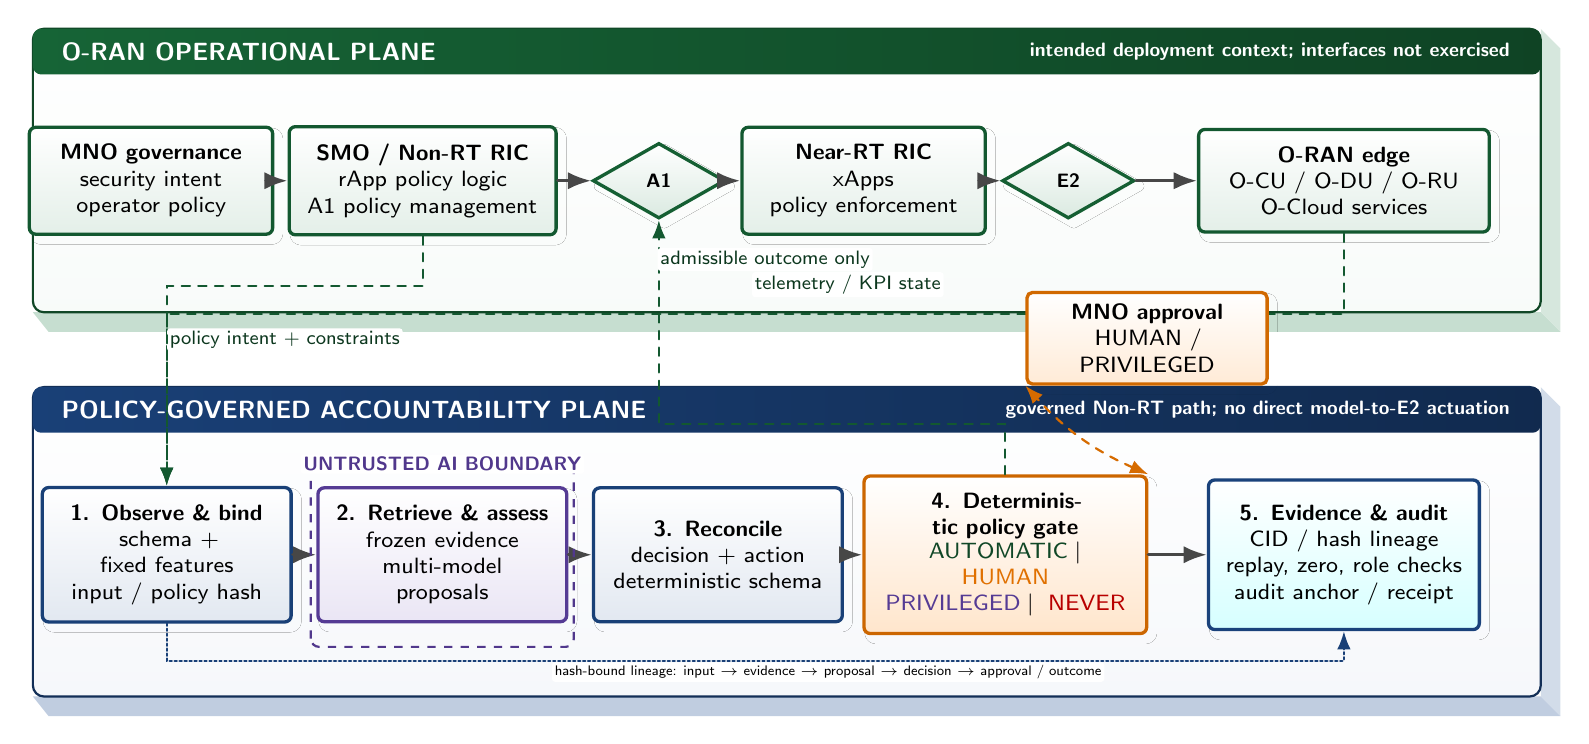
\begin{tikzpicture}[
  x=1cm,y=1cm,
  font=\sffamily\footnotesize,
  cardshadow/.style={blur shadow={shadow blur steps=5,shadow xshift=0.7mm,
    shadow yshift=-0.7mm,shadow opacity=0.22}},
  oran/.style={draw=trustgreen!72!black,very thick,rounded corners=2.3pt,
    shade,top color=white,bottom color=trustgreen!12,cardshadow,
    align=center,minimum height=10mm,text width=2.65cm,inner sep=2.2mm},
  iface/.style={draw=trustgreen!78!black,very thick,diamond,aspect=1.75,
    shade,top color=white,bottom color=trustgreen!16,cardshadow,
    align=center,minimum height=8mm,text width=1.05cm,
    font=\sffamily\scriptsize\bfseries,inner sep=0.6mm},
  stage/.style={draw=trustblue!82!black,very thick,rounded corners=2.3pt,
    shade,top color=white,bottom color=trustblue!13,cardshadow,
    align=center,minimum height=17mm,text width=2.72cm,inner sep=2.2mm},
  reason/.style={draw=toolpurple!82!black,very thick,rounded corners=2.3pt,
    shade,top color=white,bottom color=toolpurple!14,cardshadow,
    align=center,minimum height=17mm,text width=2.72cm,inner sep=2.2mm},
  gate/.style={draw=orange!80!black,very thick,rounded corners=2.3pt,
    shade,top color=white,bottom color=orange!20,cardshadow,
    align=center,minimum height=19mm,text width=3.15cm,inner sep=2.2mm},
  evidence/.style={draw=trustblue!85!black,very thick,rounded corners=2.3pt,
    shade,top color=white,bottom color=cyan!16,cardshadow,
    align=center,minimum height=19mm,text width=3.00cm,inner sep=2.2mm},
  human/.style={draw=orange!82!black,very thick,rounded corners=2pt,
    shade,top color=white,bottom color=orange!16,cardshadow,
    align=center,minimum height=8.5mm,text width=2.75cm,inner sep=1.5mm},
  flow/.style={-Latex,very thick,draw=black!72,line cap=round},
  policy/.style={-Latex,thick,dashed,draw=trustgreen!72!black,line cap=round},
  approval/.style={Latex-Latex,thick,dashed,draw=orange!84!black,line cap=round},
  bind/.style={-Latex,thick,densely dotted,draw=trustblue!82!black,line cap=round},
  layerlabel/.style={anchor=west,font=\sffamily\bfseries\small,text=white},
  mini/.style={font=\sffamily\scriptsize,align=center,inner sep=1pt}
]

% Raised O-RAN operational platform. The offset bottom/right faces provide
% restrained pseudo-3D depth while preserving vector sharpness in print.
\fill[trustgreen!25] (0.20,5.18) -- (19.40,5.18) -- (19.15,5.43) --
  (0,5.43) -- cycle;
\fill[trustgreen!18] (19.15,5.43) -- (19.40,5.18) -- (19.40,8.78) --
  (19.15,9.03) -- cycle;
\shade[top color=white,bottom color=trustgreen!3,rounded corners=4pt]
  (0,5.43) rectangle (19.15,9.03);
\draw[trustgreen!58!black,thick,rounded corners=4pt]
  (0,5.43) rectangle (19.15,9.03);
\shade[left color=trustgreen!82!black,right color=trustgreen!55!black,
  rounded corners=3pt] (0,8.45) rectangle (19.15,9.03);
\node[layerlabel] at (0.24,8.74) {O-RAN OPERATIONAL PLANE};
\node[anchor=east,font=\sffamily\scriptsize\bfseries,text=white]
  at (18.88,8.74) {intended deployment context; interfaces not exercised};

\node[oran] (mno) at (1.50,7.10)
  {\textbf{MNO governance}\\security intent\\operator policy};
\node[oran,text width=2.95cm] (smo) at (4.95,7.10)
  {\textbf{SMO / Non-RT RIC}\\rApp policy logic\\A1 policy management};
\node[iface] (a1) at (7.95,7.10) {A1};
\node[oran] (near) at (10.55,7.10)
  {\textbf{Near-RT RIC}\\xApps\\policy enforcement};
\node[iface] (e2) at (13.15,7.10) {E2};
\node[oran,text width=3.25cm] (edge) at (16.65,7.10)
  {\textbf{O-RAN edge}\\O-CU / O-DU / O-RU\\O-Cloud services};

\draw[flow] (mno) -- (smo);
\draw[flow] (smo) -- (a1);
\draw[flow] (a1) -- (near);
\draw[flow] (near) -- (e2);
\draw[flow] (e2) -- (edge);

% Raised accountability platform. Only this lower path contains LLM-based
% assessment; enforcement ownership remains outside the untrusted boundary.
\fill[trustblue!28] (0.20,0.30) -- (19.40,0.30) -- (19.15,0.55) --
  (0,0.55) -- cycle;
\fill[trustblue!20] (19.15,0.55) -- (19.40,0.30) -- (19.40,4.23) --
  (19.15,4.48) -- cycle;
\shade[top color=white,bottom color=trustblue!4,rounded corners=4pt]
  (0,0.55) rectangle (19.15,4.48);
\draw[trustblue!60!black,thick,rounded corners=4pt]
  (0,0.55) rectangle (19.15,4.48);
\shade[left color=trustblue!82!black,right color=trustblue!54!black,
  rounded corners=3pt] (0,3.90) rectangle (19.15,4.48);
\node[layerlabel] at (0.24,4.19) {POLICY-GOVERNED ACCOUNTABILITY PLANE};
\node[anchor=east,font=\sffamily\scriptsize\bfseries,text=white]
  at (18.88,4.19) {governed Non-RT path; no direct model-to-E2 actuation};

\node[stage] (observe) at (1.70,2.35)
  {\textbf{1. Observe \& bind}\\schema + fixed features\\input / policy hash};
\node[reason] (assess) at (5.20,2.35)
  {\textbf{2. Retrieve \& assess}\\frozen evidence\\multi-model proposals};
\node[stage] (reconcile) at (8.70,2.35)
  {\textbf{3. Reconcile}\\decision + action\\deterministic schema};
\node[gate] (gate) at (12.35,2.35)
  {\textbf{4. Deterministic policy gate}\\[-0.4mm]
   \textcolor{trustgreen!58!black}{AUTOMATIC}\;\textbar\;
   \textcolor{orange!88!black}{HUMAN}\\
   \textcolor{toolpurple!82!black}{PRIVILEGED}\;\textbar\;
   \textcolor{red!72!black}{NEVER}};
\node[evidence] (audit) at (16.65,2.35)
  {\textbf{5. Evidence \& audit}\\CID / hash lineage\\replay, zero, role checks\\audit anchor / receipt};

\draw[flow] (observe) -- (assess);
\draw[flow] (assess) -- (reconcile);
\draw[flow] (reconcile) -- (gate);
\draw[flow] (gate) -- (audit);

% The shaded assessment card is the only LLM-containing region.
\draw[toolpurple!78!black,dashed,thick,rounded corners=3pt]
  (3.53,1.18) rectangle (6.87,3.50);
\node[mini,font=\sffamily\scriptsize\bfseries,text=toolpurple!78!black,
  fill=white,rounded corners=1pt] at (5.20,3.50) {UNTRUSTED AI BOUNDARY};

% Cross-plane inputs and governed return. Labels sit in the inter-plane gap.
\draw[policy] (smo.south) -- ++(0,-0.63) -| (observe.north);
\node[mini,text=trustgreen!45!black,fill=white,rounded corners=1pt]
  at (3.20,5.08) {policy intent + constraints};
\draw[policy] (edge.south) -- ++(0,-1.02) -| (observe.north);
\node[mini,text=trustgreen!45!black,fill=white,rounded corners=1pt]
  at (10.35,5.78) {telemetry / KPI state};
\draw[policy] (gate.north) -- ++(0,0.64) -| (a1.south);
\node[mini,text=trustgreen!45!black,fill=white,rounded corners=1pt]
  at (9.30,6.10) {admissible outcome only};

% Human approval bridges the planes but never creates a model-to-E2 path.
\node[human] (operator) at (14.15,5.10)
  {\textbf{MNO approval}\\HUMAN / PRIVILEGED};
\draw[approval] (gate.north east) to[bend left=12] (operator.south west);

% Evidence lineage is independent of the solid decision-flow arrows and is
% kept wholly inside the accountability-plane boundary.
\draw[bind] (observe.south) -- ++(0,-0.47) -| (audit.south);
\node[mini,font=\sffamily\tiny,fill=white,rounded corners=1pt]
  at (10.10,0.86) {hash-bound lineage: input $\rightarrow$ evidence
  $\rightarrow$ proposal $\rightarrow$ decision $\rightarrow$ approval / outcome};

\end{tikzpicture}%
}
\caption{\rev{Two-plane architecture for policy-governed O-RAN security. The
operational plane depicts the intended standard SMO/Non-RT RIC--A1--Near-RT RIC--E2
path. The accountability plane binds policy and telemetry, isolates model
assessment as untrusted, reconciles proposals, applies the four-class gate,
and records the audit lineage. The SMO/A1 return is architectural and was not exercised;
HUMAN and PRIVILEGED actions require MNO approval. Models never actuate E2
directly.}}
\label{fig:architecture}
\end{figure*}
\end{revision}


\begin{revision}
\subsection{Implemented and Intended Integration}
\label{sec:integration-status}
The evaluated input is a JSON configuration with named O-RAN components and
retrieved policy evidence; it is not a standard E2 indication or a live
telemetry stream. The output is a candidate decision and action class with
hash-bound evidence. The reported prototype implements reconciliation,
policy routing and audit recording, but its action target is simulated.
Fig.~\ref{fig:architecture}'s A1/E2 path identifies intended integration.
No deployed rApp, standard A1 policy exchange, or live E2 actuation is
demonstrated. An operational adapter would need schema-validated A1 policy
instances, authenticated SMO authority, fresh target state and independently
observed application outcomes. Those are future integration requirements.
\begin{table}[!t]
\centering\ifshowrevisions\color{blue}\else\color{black}\fi\footnotesize
\caption{\rev{Component status. An implemented workflow may terminate in a simulated action.}}
\label{tab:component-status}
\begin{tabular}{p{.36\columnwidth}p{.52\columnwidth}}
\toprule
Component & Evidence status \\
\midrule
Assessment, reconciliation, audit & Implemented experimental workflow \\
HUMAN review callback & One observed approved simulation \\
Action target & Simulated ledger; no network side effects \\
Policy-gate invariants & Finite abstraction model checked \\
Oracle evaluation & Six synthetic scenarios; no expert validation \\
Public anchoring & Testnet first-inclusion experiment \\
SMO/rApp/A1/E2 deployment & Intended; not implemented in this evaluation \\
\bottomrule
\end{tabular}
\end{table}
\end{revision}
\subsection{Policy Ladder and Threat-Response Mapping}
The policy-gated control path is summarised in
Table~\ref{tab:policy-ladder}, which replaces the earlier decision-loop and
threat-response diagrams with a compact comparative structure. The central
principle is that reasoning only proposes candidate actions; execution is
mediated by the action ladder and audit anchoring. The table also maps threats to the
enforcement component and accountable outcome.
\begin{table*}[!t]
\centering
\caption{Policy ladder and threat-response mapping.}
\label{tab:policy-ladder}
\begin{adjustbox}{width=\textwidth}
\begin{tabular}{p{2.9cm}p{3.9cm}p{3.7cm}p{3.7cm}p{3.6cm}}
\toprule
Case & Input / condition & Enforcement component & Evidence path & Accountable outcome \\
\midrule
OBSERVE--REASON & Telemetry, KPI, or profile state produces a candidate action
& Telemetry and reasoning agents & Run identifier, profile metadata, local
artifact state & Candidate trust state and action proposal; no direct
actuation \\
AUTOMATIC & Low-risk action that is policy-admissible & Policy and schema
gates & Action class, admissibility check, audit record & Executed only if
admissible and audit-bound \\
HUMAN & Action requiring operator judgement & Policy ladder & Approval queue
and recorded reason & Queued for human approval; not automatically executed \\
PRIVILEGED & Action requiring stronger authority & Privileged approval
boundary & Privileged approval record and trace & Blocked from automatic
execution; requires out-of-band approval \\
NEVER & Forbidden or unsafe action & Hard policy rejection & Rejection reason
and audit trace & Blocked by construction \\
Evidence tampering & Modified evidence object or mismatched pointer & Hash/CID
and audit path & Content-addressed evidence and hash-chain continuity &
Tampered evidence is detectable and not silently trusted \\
Replay attempt & Duplicate prior commitment & Smart-contract duplicate check &
Existing commitment and rejection event & Replayed commitment is rejected \\
Zero-anchor attempt & Empty or zero commitment & Smart-contract invariant &
Non-zero commitment check & Zero commitment is rejected \\
Unauthorised submitter & Submitter lacks authority & Role/capability gate &
Submitter identity and rejection event & Unauthorised submission is rejected \\
\bottomrule
\end{tabular}
\end{adjustbox}
\end{table*}
\subsection{Smart-Contract Boundary}
The smart contract does not control radio traffic directly. Its role is
limited to audit accountability: storing compact commitments, rejecting
duplicate commitments, rejecting zero commitments, and enforcing authorised
submitters. It cannot guarantee IPFS availability, prove physical network
truth, or replace MNO operational policy. This boundary avoids overclaiming:
the ledger records and verifies governance evidence, while the O-RAN control
plane remains responsible for real network execution.

\begin{revision}
The archived HUMAN demonstration's ANCHORED status denotes a local hash-chain
record: its external-chain evidence field is MISSING. Its audit record must
not be conflated with the separate 90-pair public-testnet experiment. Inclusion
of a commitment cannot establish telemetry truth, availability of off-chain
evidence, key security or economic finality. Those assumptions remain outside
the measured latency study.
\end{revision}

\begin{revision}
\section{Formal Safety Analysis}
\label{sec:formal}
The executable TLA+ gate has state fields \texttt{phase}, \texttt{actionClass},
\texttt{humanApproved}, \texttt{privilegedApproved}, \texttt{proofValid},
\texttt{anchorCommitment} and \texttt{executed}. Its six invariants state:
NEVER implies no execution; executed HUMAN requires human approval;
executed PRIVILEGED requires both approval Booleans; execution requires
abstract admissibility and a non-zero commitment; and execution implies
the ACT phase. The corresponding identifiers are \texttt{NeverNotExecuted},
\texttt{HumanRequiresApproval}, \texttt{PrivilegedRequiresBoth},
\texttt{ProofRequired}, \texttt{NonZeroAnchorRequired} and
\texttt{NoExecutionBeforeAct}. Exact predicates are given in the supplement.
\texttt{proofValid} denotes abstract admissibility, not a successfully
verified cryptographic proof. Approval Booleans are assumptions about state,
not a verified human-authentication protocol.

We reproduced TLC~2.19's original 64 initial states, 320 reachable states,
depth five and zero invariant violations~\cite{lamportTla}. Its initial
predicate excludes zero commitments, making the non-zero property
unexercised on zero inputs. A separate revision probe admits zero, yielding
96 initial and 480 reachable states with no invariant violation. Three
mutations removing admissibility, the non-zero execution guard, or HUMAN
approval for PRIVILEGED each produce the expected counterexample. The
original model is preserved. It contains no history of accepted commitments:
duplicate-anchor rejection is runtime/contract evidence, not a TLC result.
Neither run proves liveness, code refinement, model semantic correctness,
asynchronous RAN safety or production deployment safety. ACT/BLOCK are
terminal; \texttt{-deadlock} suppresses terminal-state warnings and does not
establish termination. Logs and model hashes accompany the revision.
\end{revision}

\section{Reproducible Evaluation Methodology}
\label{sec:methodology}
\subsection{Staged Evaluation}
Six stages progressively add evidence: (1) the response
matrix, KPI plan, executable TLA\textsuperscript{+} model, and n8n skeleton;
(2) the clean
240-record workflow matrix; (3) anchor, reasoning, and negative-security
runtime hooks; (4) Sepolia validation; (5) the paired PoS--Roll-DPoS and local
hash-primitive studies; and (6) three real etcd/Raft and Besu/QBFT
permissioned-cluster sessions. The paper harness additionally performs
packet-capture smoke testing, AUTH\_V2.2 timing, AI-evidence diagnostics,
Stage~F/F row hashing, and evidence-manifest generation.
\subsection{Paired PoS--Roll-DPoS Consensus-Sensitivity Study}
The Stage~5 experiment asks a deliberately bounded question: when identical
\texttt{Stage3AnomalyLedger} runtime bytecode receives matched audit-anchor
transactions at approximately the same time, how do client-observed
first-inclusion latency, EVM execution gas, and observed block cadence differ
between Ethereum Sepolia and IoTeX testnet? Sepolia uses chain ID 11155111
and the Ethereum PoS protocol, but its permissioned test validator set
prevents extrapolation to Ethereum mainnet~\cite{ethereumNetworks}. IoTeX
testnet uses chain ID 4690, exposes an Ethereum-compatible JSON-RPC endpoint,
and runs Roll-DPoS~\cite{iotexRollDpos,iotexRpc}.
The Solidity 0.8.20 contract is compiled once (optimizer 200,
\texttt{viaIR=true}). Each session verifies both chain IDs, deploys the same
creation bytecode, checks non-empty deployed code, and requires identical
runtime-code Keccak-256 hashes across networks and sessions. After three
excluded warm-up pairs, each session executes 30 measured pairs; pair $(s,i)$
carries the same commitment and evidence digest on both networks, submitted
concurrently from the same client host, so three sessions provide
$N = 3\times 30 = 90$ pairs. The client host, per-network RPC provider,
compiler settings, bytecode, gas limit, and one-confirmation receipt rule
remain fixed.
For network $n \in \{S, I\}$, where $S$ denotes Sepolia and $I$ denotes IoTeX,
the primary observation is
\begin{equation}
L^{(n)}_{s,i} = t^{(n)}_{s,i,\mathrm{receipt}} - t^{(n)}_{s,i,\mathrm{submit}}.
\label{eq:latency}
\end{equation}
This interval begins immediately before the JSON-RPC transaction submission
and ends when a successful receipt is available after one inclusion. It
includes client/RPC overhead, propagation, producer waiting time, and
prevailing public-testnet load; it is not economic-finality latency. The
paired estimands use the same orientation:
\begin{equation}
\Delta_{s,i} = L^{(S)}_{s,i} - L^{(I)}_{s,i}, \qquad
R_{s,i} = \frac{L^{(S)}_{s,i}}{L^{(I)}_{s,i}}.
\label{eq:estimands}
\end{equation}
Both estimands are summarised by their medians over pairs; the reported ratio
is therefore a median of per-pair ratios and is not expected to equal the
quotient of the two marginal medians. The harness also records deployment and
anchor gas, effective gas price, transaction and block identifiers,
receipt/event integrity, and at least 64 consecutive post-run block headers
per session. Duplicate, zero-commitment, and unauthorised-submitter checks run
as read-only \texttt{eth\_call} probes against each deployed state, testing
rejection semantics without mining deliberately reverting transactions;
native-token gas prices are retained for provenance only.
The deterministic analysis reports medians, quartiles, P95, means, and sample
standard deviations using R-7 linear-interpolated quantiles. Median intervals
use 10{,}000 replicates of a two-level hierarchical bootstrap with fixed seed
20260721: sessions are resampled first and matched pairs are resampled within
each selected session. This preserves the session-clustered design. The
publication gate fails closed for fewer than three sessions, fewer than 30
measured pairs per session, wrong chain IDs, bytecode mismatch, unsuccessful
receipts, missing anchor events, or any failed rejection probe. Each raw
\texttt{benchmark.json} has a companion \texttt{SHA256SUMS.txt}; a derivation
manifest binds the three input hashes to the generated summary, table, figure,
and results paragraph.
Because only three session clusters are available, the bootstrap intervals are
descriptive summaries of the retained sessions; reliable nominal 95\%
coverage is not claimed.
\subsection{Permissioned Raft--QBFT Fault Experiment}
Pinned etcd~3.5.17 and Besu~24.5.4 clients run a real three-member Raft
cluster and four-validator QBFT network, respectively
~\cite{ongaro2014raft,besuQbft,artifactRepo}. Three clean sessions retain 30
observations per latency condition ($n=90$). Raft is tested healthy, with one
follower stopped, after leader failover, without a majority, and after
restoration. QBFT is tested healthy, with 3/4 and 2/4 validators, and after
operator-assisted restoration; the 2/4 case records bounded block-height
probes, not transaction latency. Publication requires correct identities and
counts, expected progress/non-progress, contract/event integrity, clean Git
state, and valid SHA-256 manifests. Because Raft measures etcd key/value
replication while QBFT executes \texttt{Stage3AnomalyLedger}, latency is
compared only within each family. Injected faults are process
crash/non-participation and quorum loss, not equivocation, forged votes,
state corruption, or arbitrary Byzantine messages.
\begin{revision}
\subsection{Frozen Synthetic-Policy Oracle Benchmark}
\label{sec:oracle-method}
The retrieval comparison is evaluated through a separate, frozen oracle
benchmark rather than being merged with the 240-record impairment-profile
matrix. The benchmark crosses six synthetic O-RAN policy scenarios with three
retrieval modes---No RAG, RAG, and Agentic RAG---and ten recorded
repetitions, giving $6\times3\times10 = 180$ canonical successful cells. Each
cell is evaluated against the same executable synthetic operator-policy
oracle. Freezing the oracle, prompts, scenario payloads, and metric definitions
before aggregation prevents post-hoc relabelling; the oracle is an
experimental reference function, not expert-verified ground truth or a claim
of comprehensive O-RAN/3GPP compliance.
The execution design separates semantic population from operational
attempts: the semantic denominator contains one successful package per
planned cell, while an append-only attempt index retains every invocation,
including failed workflow-boundary attempts, and SUCCESS-only resumption
retries incomplete cells without deleting prior failures. The 233 operational
attempts (180 successes, 53 retained HTTP-500 failures) therefore measure
workflow reliability and resumability, whereas the 180 successful cells
measure oracle-relative behaviour; $180/233$ is not model accuracy or a
final-cell completion rate.
Whole-scenario percentile intervals use 20{,}000 fixed-seed bootstrap
replicates over the six scenario clusters. Repeats assess within-cell
stability, not independent scenario-level generalisation. Independent human
validation was not conducted because eligible annotators were unavailable;
the frozen oracle will not be revised in response to any future labels.
Fig.~\ref{fig:five-stage-pipeline} presents the five-stage path used for the
oracle benchmark and live demonstration: observe, propose, govern, bind, and
audit. The supplement retains the complete exported canvas, node identifiers,
and archived execution trace.

\begin{revision}
\begin{figure*}[t]
\centering
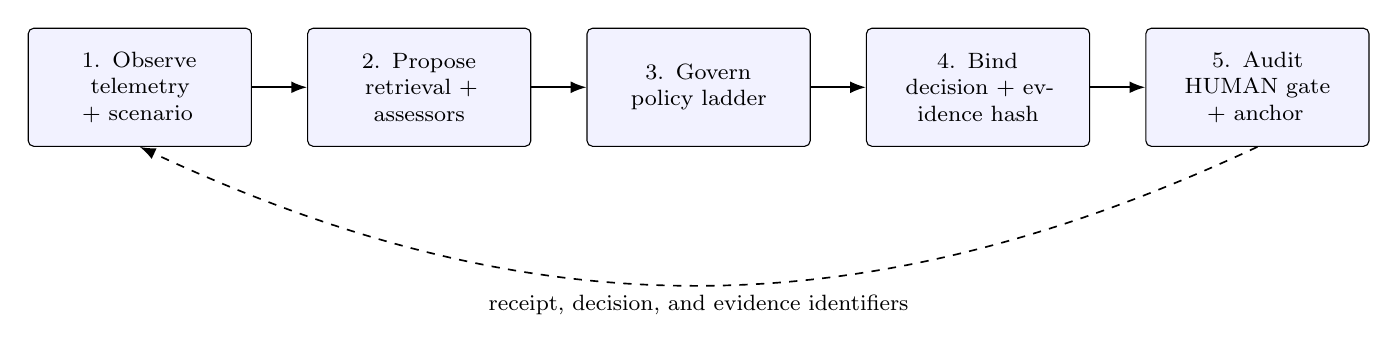
\begin{tikzpicture}[
  font=\footnotesize,
  stage/.style={draw,rounded corners=2pt,align=center,text width=2.6cm,
    minimum height=15mm,fill=blue!5},
  flow/.style={-Latex,semithick},
  node distance=7mm
]
\node[stage] (observe) {1. Observe\\telemetry + scenario};
\node[stage,right=of observe] (reason) {2. Propose\\retrieval + assessors};
\node[stage,right=of reason] (govern) {3. Govern\\policy ladder};
\node[stage,right=of govern] (bind) {4. Bind\\decision + evidence hash};
\node[stage,right=of bind] (audit) {5. Audit\\HUMAN gate + anchor};
\draw[flow] (observe) -- (reason);
\draw[flow] (reason) -- (govern);
\draw[flow] (govern) -- (bind);
\draw[flow] (bind) -- (audit);
\draw[flow,dashed] (audit.south) to[bend left=25]
  node[below]{receipt, decision, and evidence identifiers} (observe.south);
\end{tikzpicture}
\caption{\rev{Five-stage execution schematic. Model output remains untrusted until
the external policy ladder admits it. The complete exported workflow and its
node-level configuration are provided in the supplement.}}
\label{fig:five-stage-pipeline}
\end{figure*}
\end{revision}

For each retrieval mode $m$, let $N_m = 60$, let $d_i$ be the final decision,
$a_i$ the enforced action class, and $(d^{\star}_i, a^{\star}_i)$ the frozen
oracle labels. Let $z_i = 1$ denote a covered, non-abstaining output. The
principal oracle-relative metrics are
{\small
\begin{align}
\mathrm{AD}(m) &= \tfrac{1}{N_m}\textstyle\sum_i \mathbf{1}[d_i = d^{\star}_i], &
\mathrm{AA}(m) &= \tfrac{1}{N_m}\textstyle\sum_i \mathbf{1}[a_i = a^{\star}_i], \\
\mathrm{C}(m)  &= \tfrac{1}{N_m}\textstyle\sum_i z_i, &
\mathrm{AS}(m) &= \frac{\sum_i z_i\,\mathbf{1}[d_i = d^{\star}_i]}{\sum_i z_i}.
\end{align}
}
Here, AD is decision agreement, AA is enforced-action agreement, C is coverage,
and AS is selective decision agreement. Abstention is $1-\mathrm{C}$.
Safe-given-abstention is calculated over abstaining cells and reports whether
the enforced route remained fail-closed. If $\sum_i z_i = 0$, selective
agreement is undefined and reported as N/A. Provider and role-chain validation
are deterministic artifact checks and are reported separately from
oracle-relative semantic agreement.

\begin{revision}
\paragraph{Scenario construction and limits}
The frozen configurations are author-designed policy cases, not sampled
operator incidents. Table~\ref{tab:scenario-map} maps their exact fields to
O-RAN management concerns. P-01--P-04 are clauses of an explicitly
experimental operator policy, not normative O-RAN clause identifiers. The
oracle assigns HUMAN even to compliant S1: its label encodes a review policy,
not permission for autonomous execution. None of the six reference classes
is AUTOMATIC or PRIVILEGED. The benchmark therefore does not assess useful
automatic execution or the full four-class distribution.
\begin{table}[!t]
\centering\ifshowrevisions\color{blue}\else\color{black}\fi\footnotesize
\caption{\rev{Frozen scenarios and oracle labels. C/NC/U denote COMPLIANT,
NON\_COMPLIANT and UNCERTAIN; H/N denote HUMAN and NEVER.}}
\label{tab:scenario-map}
\begin{tabular}{cp{.57\columnwidth}cc}
\toprule ID & Configuration and management concern & Decision & Class \\
\midrule
S1 & O-CU/O1; NEA2, NIA2, integrity enabled, TLS 1.3 & C & H \\
S2 & O-CU/F1-U; integrity disabled despite required MNO profile (P-01) & NC & H \\
S3 & SMO--O-CU/O1; TLS 1.0 compatibility request (P-02) & NC & H \\
S4 & Near-RT RIC/E2; unregistered xApp, RBAC false (P-03) & NC & N \\
S5 & Audit service; duplicate prior commitment (P-04) & NC & N \\
S6 & O-DU; unverified summary, unknown interface, absent security profile & U & H \\
\bottomrule
\end{tabular}
\end{table}
Missing evidence is explicit in S6, and S2/S4 contain a request conflicting
with policy. Retrieved distractors and the two reconciliation mismatches are
recorded, but this is not a systematic noisy-telemetry or adaptive-conflict
study. The separate delay/jitter/loss experiment configures workflow stress;
it does not measure radio-channel realism. Independent expert labels,
production-derived scenarios and held-out noise/conflict validation remain
absent. We narrow the conclusions accordingly and preserve the frozen oracle.
\end{revision}
\end{revision}
\subsection{Artifact Reproducibility}
\rev{The historical public artifact is version~1.0.0~\cite{artifactRepo}.
The revision-specific reproducibility archive adds the marked/clean sources,
unchanged retained-data packages, reanalysis code, formal logs and editable
figures. Its build information identifies the repository commit and file
digests. These new checks must not be attributed to the older DOI release.
The supplement describes the evidence objects and reproduction commands.
Baseline metrics are recomputed from retained records; proposed-workflow
counts are checked against archived scenario histograms. The original 180
proposed per-cell packages are not included in this revision archive, so the
revision does not claim to have rerun their complete raw-output analysis.}
\subsection{Claim Boundary}
\label{sec:claim-boundary}
Claims are restricted to the released implementation and retained evidence.
TLC establishes six invariants only for the finite model and explored state
space. Oracle metrics measure agreement with a frozen synthetic reference, not
expert-verified or population-level accuracy. Public-testnet results measure
client-observed first inclusion and include RPC, propagation, cadence, load,
and chain-policy effects; they do not measure economic finality or isolate
consensus. The permissioned faults cover crash/non-participation, not arbitrary
Byzantine behaviour. The live n8n path uses simulated actuation and a simulated
ledger and does not establish production O-RAN integration, availability, or
safety. Cross-provider observations apply to the recorded aliases, prompts,
and access dates and need not persist after provider updates.
The frozen 240-row matrix has no per-row proof outcome or
proof/public-input binding and therefore supports 0/240 row-bound successful
verifications. AUTH\_V2.2 is reported only as a component experiment,
including its observed \texttt{verifyTx=false} outcome; no system-level
zero-knowledge claim is made. Prompt-injection and open-weights results are
likewise confined to their specified synthetic suites. n8n coordinates
experiments but remains outside the trusted computing base.
Table~\ref{tab:eval-matrix} summarises the denominators.
\begin{table}[!t]
\centering
\caption{Evaluation matrix and evidence outputs.}
\label{tab:eval-matrix}
\begin{adjustbox}{width=\columnwidth}
\begin{tabular}{p{2.6cm}p{5.6cm}}
\toprule
Dimension & Values \\
\midrule
Variants & Full system, no AUTH, oracle-only, RBAC-only, no IPFS, no policy gate \\
Profiles & Clean, delay, delay+jitter, delay+jitter+loss \\
Repeats & 10 per variant/profile pair \\
Core records & $6\times4\times10 = 240$ local clean records \\
Oracle benchmark & 6 scenarios $\times$ 3 retrieval modes $\times$ 10 repeats
= 180 successful cells \\
External baseline & LangGraph: the same 180 frozen cells; 180/180 HTTP~200 \\
Open weights & Qwen3-4B: 60 Agentic-RAG cells; local Ollama endpoint \\
Injection suite & 10 attack families $\times$ 3 base contexts = 30 cases \\
Operational attempts & 233 append-only attempts: 180 successful and 53
retained HTTP-500 failures \\
Consensus sensitivity & 3 sessions $\times$ 30 measured pairs = 90; 9 warm-up
pairs excluded \\
Permissioned faults & 3 sessions; 90 retained observations per latency
condition and 90 quorum-loss probes per implementation \\
Block-cadence sample & 189 consecutive intervals per network across the three
sessions \\
Hash microbenchmark & 3 primitives $\times$ 2 payload sizes $\times$ 30
retained \texttt{eth\_call} observations (3 warm-ups excluded per cell) \\
Formal verification & TLC 2.19; 64 initial states, 320 distinct reachable
states, depth 5, six invariants \\
Outputs & Run ID, Git hash, raw logs, evidence hashes, KPI JSON/CSV,
claim-validation report, evidence manifest \\
\bottomrule
\end{tabular}
\end{adjustbox}
\end{table}
\subsection{AI-Assisted n8n Workflow Extension}
\label{sec:n8n-extension}
Additional Stage~E/F and Stage~F/F orchestration observations are moved to the
supplement. Their small, selectively valid samples are not used for the
principal effectiveness or generalisability claims. The oracle benchmark uses
GPT-5.6 as an assessor; the distinct GPT-5.5 alias appears only as the planner
in the supplemental Stage~F/F workflow.
\section{Results and Discussion}
\label{sec:results}

\begin{revision}
\paragraph{Operational timescale and intended use}
The recorded 80.453--109.793~s medians and 164.747~s Agentic-RAG P95 exclude
Near-RT control and urgent inline containment. Non-RT positioning alone does
not validate a deadline. Candidate tasks are policy-change preparation,
compliance review and scheduled remediation planning, subject to an
operator-approved budget above the observed tail and evidence-freshness
checks. No task-specific service-level objective is validated here. Human
waiting follows recommendation generation and must be budgeted separately.
When a deadline or evidence lifetime expires, a deployment should withhold
actuation and require fresh assessment; that expiry behaviour is a requirement,
not an observed production property.
\end{revision}

\subsection{Live n8n Execution and Human-Governed Outcome}
\label{sec:live-run}
To distinguish architectural intent from observed execution, the final-paper
production workflow was exercised as a live supervisor demonstration using
scenario S2 (DRB integrity disabled) in AGENTIC\_RAG mode. The production
webhook returned HTTP 200, and n8n recorded successful master execution
\#1412 in 109.436\,s for run
\texttt{d7c0e31b-fa9e-437b-87d2-acdeef4a6ba1}, with a NON\_COMPLIANT
decision and the HUMAN action class enforced. Four of four provider stages
and four of four agent-role stages passed the artifact checks, after which
the report reached the ANCHORED state. Execution \#1412 traverses the
five-stage workflow of Fig.~\ref{fig:five-stage-pipeline}: input binding,
retrieval, independent provider assessment, consensus, the
planner--critic--recovery--arbiter chain, policy and formal-evidence gates,
audit anchoring, and governed-action preparation. (The n8n UI shows
host-local BST while evidence files use UTC; the one-hour offset is expected
and does not denote a second run.)
Fig.~\ref{fig:human-gate-state-machine} isolates the governance transition. A
separate callback first validates the reviewer payload, then submits the
authorised decision to the gateway. Execution \#1417 completed successfully in
39\,ms and followed the \emph{true} branch of \emph{Review Approved?}; the
rejection branch remained unexecuted. The gateway subsequently recorded
APPROVE and SIMULATED\_EXECUTED for the governed action. Crucially, approval
did not authorise production actuation: the execution target was
\texttt{SIMULATED\_O\_RAN\_ACTION\_LEDGER},
\texttt{production\_oran\_execution} was \texttt{false}, and
\texttt{network\_side\_effects} was \texttt{false}. The split between the main
workflow and review callback therefore operationalises the HUMAN class as a
distinct, auditable control transition rather than an implicit continuation of
model reasoning.

\begin{revision}
\begin{figure}[t]
\centering
\resizebox{\columnwidth}{!}{%
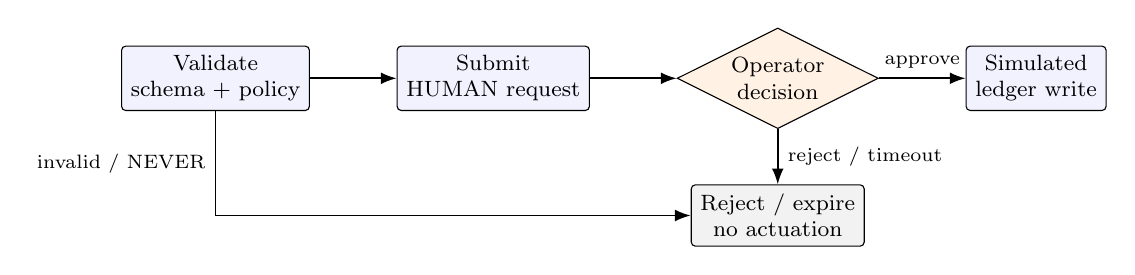
\begin{tikzpicture}[
  font=\footnotesize,
  node distance=7mm and 11mm,
  state/.style={draw,rounded corners=1.5pt,align=center,minimum height=7mm,
    minimum width=16mm,fill=blue!5},
  terminal/.style={draw,rounded corners=1.5pt,align=center,minimum height=7mm,
    minimum width=16mm,fill=gray!10},
  guard/.style={draw,diamond,aspect=2.0,align=center,inner sep=1.5pt,
    fill=orange!10},
  flow/.style={-Latex,semithick}
]
\node[state] (validate) {Validate\\schema + policy};
\node[state,right=of validate] (submit) {Submit\\HUMAN request};
\node[guard,right=of submit] (decision) {Operator\\decision};
\node[state,right=of decision] (ledger) {Simulated\\ledger write};
\node[terminal,below=of decision] (stop) {Reject / expire\\no actuation};
\draw[flow] (validate) -- (submit);
\draw[flow] (validate) |- node[pos=.25,left,font=\scriptsize]{invalid / NEVER} (stop);
\draw[flow] (submit) -- (decision);
\draw[flow] (decision) -- node[above,font=\scriptsize]{approve} (ledger);
\draw[flow] (decision) -- node[right,font=\scriptsize]{reject / timeout} (stop);
\end{tikzpicture}
}
\caption{\rev{HUMAN-gate state transition. The approved simulated-ledger branch was observed.
Invalid, reject and timeout branches show intended fail-closed requirements;
complete branch coverage is not claimed.}}
\label{fig:human-gate-state-machine}
\end{figure}
\end{revision}

The visual trace is cross-bound to machine-verifiable artifacts rather than
treated as primary proof. The full report and governed-action SHA-256 digests
are retained in the artifact; their prefixes/suffixes are
\texttt{8a36aed6\ldots f4b65e9} and \texttt{4a345bb1\ldots f7124d18}.
Fourteen consistency conditions over the report and review response passed,
and the evidence directory includes a recursively verified SHA-256 manifest.
Consequently, the machine-readable artifacts establish that the documented
workflow executed and traversed the HUMAN gate. Its interpretation is governed
by the Claim Boundary in Section~\ref{sec:claim-boundary}.

\begin{revision}
\paragraph{Operator authority and review boundary}
The archived callback records a reviewer identifier, claimed role, Boolean
decision and rationale, with run and report hashes linking the pending action
to its outcome. The HUMAN role is an MNO approver; PRIVILEGED denotes an
additional authority requirement, with both approval Booleans required by
the formal abstraction. A recorded identifier/role is not evidence of
cryptographic reviewer authentication. The retained positive callback and
simulated write establish one transition only: reject, expiry, replay,
concurrent decisions and approval revocation are not empirically established.

A deployment approval view should expose the exact action and target, policy
version, supporting evidence and uncertainty. An authenticated decision should
bind the action/evidence version and include identity, authority, timestamp,
reason and expiry. Conflicting decisions, stale evidence or changed payloads
should leave the action blocked until a fresh authorised decision. These
remain deployment requirements. A new inactive callback export corrects
Boolean string coercion with strict validation; local payload tests do not
demonstrate gateway authentication or deployed approval enforcement.
\end{revision}

\begin{revision}
\subsection{Frozen Oracle Benchmark Performance}
Table~\ref{tab:oracle-results} reports the complete oracle-relative comparison
over 180 canonical successful cells, with 60 cells per retrieval mode. The
results show a monotonic improvement in decision agreement and coverage as
retrieval structure increases. No RAG achieves only 16.7\% decision agreement
and zero coverage because every cell is marked as an abstention. Its 66.7\%
action agreement and 100\% safe-given-abstention rate indicate that the
governance layer frequently selected a conservative action despite the absence
of a covered semantic decision. This behaviour is safe but operationally
uninformative.

\begin{revision}
\begin{table*}[!t]
\centering\ifshowrevisions\color{blue}\else\color{black}\fi
\caption{\rev{Agreement with the frozen synthetic oracle and proposed-workflow
coverage. Each mode has six scenarios and ten repeats ($n=60$). Bracketed
scenario-clustered bootstrap intervals are descriptive; they do not validate
O-RAN correctness or generalisation.}}
\label{tab:oracle-results}
\begin{tabular}{lrrr}
\toprule Mode & Decision agreement (\%) & Enforced-action agreement (\%) & Coverage (\%) \\
\midrule
No RAG & 16.7 [0.0, 50.0] & 66.7 [33.3, 100.0] & 0.0 [0.0, 0.0] \\
RAG & 83.3 [50.0, 100.0] & 83.3 [50.0, 100.0] & 66.7 [33.3, 100.0] \\
Agentic RAG & 100.0 [100.0, 100.0] & 96.7 [93.3, 100.0] & 83.3 [50.0, 100.0] \\
\bottomrule
\end{tabular}
\end{table*}
\end{revision}

RAG raises decision and enforced-action agreement to 83.3\%, with 66.7\%
coverage and 33.3\% abstention. Agentic RAG reaches 100.0\% decision agreement,
96.7\% enforced-action agreement, and 83.3\% coverage. Both retrieval modes
achieve 100.0\% selective agreement on covered cells and 100.0\% safety
conditional on abstention. Therefore, the gain is not obtained by forcing a
decision in every case: the workflow retains a measurable abstention channel
and keeps abstaining cases fail-closed.
Decisions were repeat-stable in all 18 scenario--mode groups; enforced actions
were stable in 16/18. Agentic-RAG S2 produced HUMAN in nine repeats and NEVER
in one, while S4 produced NEVER in nine and HUMAN in one. Ten repeats do not
create 60 independent scenarios. With only six clusters, the 20{,}000-replicate
intervals are descriptive and reliable nominal coverage is not claimed.
Fig.~\ref{fig:composite-oracle-results}(a) visualises the principal semantic
metrics.
The difference between Agentic-RAG decision agreement (100.0\%) and action
agreement (96.7\%) is important: the final semantic decision matched the oracle
for every cell, but deterministic evidence reconciliation changed the enforced
class in two of 60 cells. Fig.~\ref{fig:composite-oracle-results}(d) shows the
associated latency cost. Relative to No RAG, RAG increases median latency by
19.699\,s (24.5\%) and P95 latency by 42.016\,s (38.6\%). Agentic RAG
increases the median by a further 9.641\,s and P95 by 13.978\,s. End-to-end,
Agentic RAG is 36.5\% slower at the median and 51.5\% slower at P95 than No
RAG. The benchmark therefore supports an agreement--coverage--latency trade-off
rather than an unqualified claim that the most agentic mode is superior for
every operational objective.

\begin{revision}
\begin{figure*}[t]
\centering
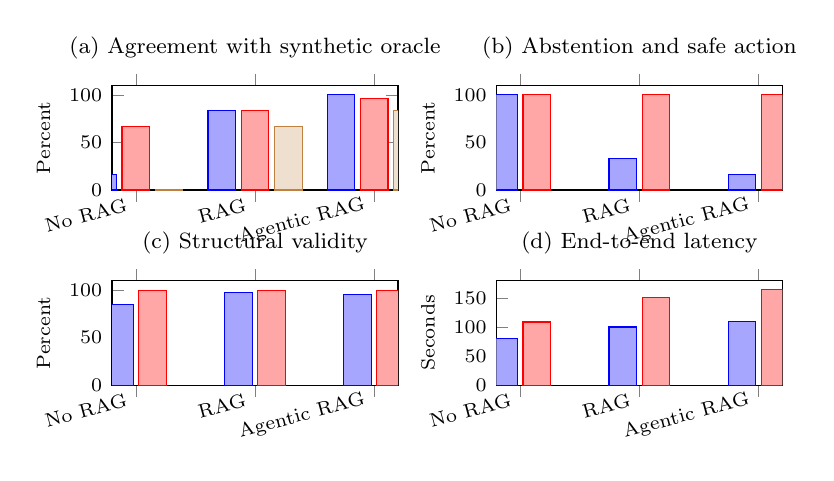
\begin{tikzpicture}
\begin{groupplot}[
  group style={group size=2 by 2,horizontal sep=1.25cm,vertical sep=1.15cm},
  width=.43\textwidth,height=.24\textwidth,ybar,
  symbolic x coords={No RAG,RAG,Agentic RAG},xtick=data,
  x tick label style={rotate=15,anchor=east,font=\scriptsize},
  tick label style={font=\scriptsize},label style={font=\scriptsize},
  title style={font=\footnotesize},ymin=0,ymax=110,ylabel={Percent}
]
\nextgroupplot[title={(a) Agreement with synthetic oracle}]
  \addplot[fill=blue!35,draw=blue] coordinates {(No RAG,16.7) (RAG,83.3) (Agentic RAG,100.0)};
  \addplot[fill=red!35,draw=red] coordinates {(No RAG,66.7) (RAG,83.3) (Agentic RAG,96.7)};
  \addplot[fill=brown!25,draw=brown] coordinates {(No RAG,0.0) (RAG,66.7) (Agentic RAG,83.3)};
\nextgroupplot[title={(b) Abstention and safe action}]
  \addplot[fill=blue!35,draw=blue] coordinates {(No RAG,100.0) (RAG,33.3) (Agentic RAG,16.7)};
  \addplot[fill=red!35,draw=red] coordinates {(No RAG,100.0) (RAG,100.0) (Agentic RAG,100.0)};
\nextgroupplot[title={(c) Structural validity}]
  \addplot[fill=blue!35,draw=blue] coordinates {(No RAG,85.0) (RAG,97.9) (Agentic RAG,95.8)};
  \addplot[fill=red!35,draw=red] coordinates {(No RAG,100.0) (RAG,100.0) (Agentic RAG,100.0)};
\nextgroupplot[title={(d) End-to-end latency},ylabel={Seconds},ymin=0,ymax=180]
  \addplot[fill=blue!35,draw=blue] coordinates {(No RAG,80.453) (RAG,100.152) (Agentic RAG,109.793)};
  \addplot[fill=red!35,draw=red] coordinates {(No RAG,108.753) (RAG,150.769) (Agentic RAG,164.747)};
\end{groupplot}
\end{tikzpicture}
\par\smallskip
{\scriptsize
\begin{tabular}{@{}p{.47\textwidth}@{\hspace{.03\textwidth}}p{.47\textwidth}@{}}
(a) \textcolor{blue}{Decision agreement}; \textcolor{red}{action agreement}; \textcolor{brown}{coverage} &
(b) \textcolor{blue}{Abstention}; \textcolor{red}{safe given abstention} \\
(c) \textcolor{blue}{Provider validity}; \textcolor{red}{role validity} &
(d) \textcolor{blue}{Median}; \textcolor{red}{P95}
\end{tabular}}
\caption{\rev{Consolidated frozen-oracle results ($60$ cells per mode). Agreement is
relative to six synthetic scenarios. Safe routing and structural validation
do not establish semantic correctness. Latency is reported separately; no
operational deadline is validated, and Near-RT use is excluded.}}
\label{fig:composite-oracle-results}
\end{figure*}
\end{revision}

Table~\ref{tab:mismatch} diagnoses the two Agentic-RAG action-class
mismatches. In S2 repeat 10, unsupported P-03 evidence was retained together
with P-01, so deterministic reconciliation escalated HUMAN to NEVER. This
error is over-restrictive and preserves safety because automatic execution
remains disabled. In S4 repeat 5, exact P-03 evidence was not retained and the
final clauses became UNSPECIFIED, so reconciliation downgraded the model
proposal from NEVER to HUMAN. Although this direction is under-restrictive
relative to the oracle, HUMAN still requires explicit review and therefore
remains fail-closed. These two cases explain the $58/60 = 96.7\%$ action
agreement while automatic execution remained disabled in this benchmark.
\begin{table}[!t]
\centering
\caption{Agentic-RAG action-class mismatch diagnosis. Both mismatches remained fail-closed.}
\label{tab:mismatch}
\footnotesize
\begin{adjustbox}{width=\columnwidth}
\begin{tabular}{p{1.2cm}p{1.7cm}p{2.6cm}p{2.6cm}}
\toprule
Cell & Oracle / enforced & Evidence-boundary cause & Safety outcome \\
\midrule
S2, r10 & HUMAN / NEVER (over-restrictive) & Unsupported P-03 retained with
P-01; reconciliation escalated the action. & OPA enforced NEVER; automatic
execution remained disabled. \\
S4, r5 & NEVER / HUMAN (under-restrictive) & Exact P-03 evidence not
retained; final clauses UNSPECIFIED; reconciliation downgraded the NEVER
proposal. & OPA enforced HUMAN; path remained fail-closed and required
review. \\
\bottomrule
\end{tabular}
\end{adjustbox}
\end{table}
\end{revision}

\begin{revision}
\subsection{External and Open-Weights Baselines}
The external LangGraph baseline used version 1.2.10, the same canonical
180-cell JSONL (SHA-256
\texttt{4854f1d4\ldots e1196c6c}), the same scenario labels and scoring, and
one assessor node followed by deterministic reconciliation. All 180 requests
returned HTTP~200. Temperature was 0, top-$p$ was 1, and the completion limit
was 256 tokens; the endpoint returned the requested
\texttt{gpt-5.6-terra} alias. Table~\ref{tab:external-baseline} replaces a
qualitative tick comparison with measured results.
\begin{table*}[!t]
\centering\ifshowrevisions\color{blue}\else\color{black}\fi
\caption{\rev{Quantitative baselines on the frozen oracle. CIs in
Table~\ref{tab:oracle-results} apply only to the proposed-system rows.}}
\label{tab:external-baseline}
\scriptsize
\begin{tabular}{llrrrrr}
\toprule
System & Mode / cells & Decision agreement & Action agreement & Joint agreement &
NEVER recall & Recorded median (s) \\
\midrule
LangGraph & No RAG / 60 & 83.3\% & 66.7\% & 50.0\% & 100.0\% & 1.487~s \\
LangGraph & RAG / 60 & 83.3\% & 66.7\% & 50.0\% & 100.0\% & 1.683~s \\
LangGraph & Agentic RAG / 60 & 83.3\% & 66.7\% & 50.0\% & 100.0\% & 1.843~s \\
Proposed system & Agentic RAG / 60 & 100.0\% & 96.7\% & 96.7\% &
95.0\% & 109.793~s \\
Qwen3-4B local & Agentic RAG / 60 & 63.3\% & 18.3\% & 11.7\% &
55.0\% & 238.381~s \\
\bottomrule
\end{tabular}
\end{table*}
For all systems, NEVER recall is the fraction of oracle-NEVER cases whose
final action class is NEVER; it is distinct from an execute-true flag. The
retained repeat counts give proposed Agentic-RAG recall $19/20=95.0\%$:
S4 has nine NEVER and one HUMAN result, while S5 has ten NEVER results.
The HUMAN mismatch remains an action-class error even with automatic
execution disabled. This corrects the previous table's 100.0\% entry.
The LangGraph baseline recorded zero NEVER-boundary bypass flags and zero unsafe execution declarations; its estimated API cost was USD~0.856704. The open-weights run used
Qwen3-4B Q4\_K\_M through Ollama~0.12.3 on CPU~\cite{qwen3}, with digest
\texttt{359d7dd4\ldots 94fae7}, seed 20260808, temperature 0, top-$p$ 1,
top-$k$ 20, a 16{,}384-token context window, and a 256-token completion limit.

\begin{revision}
It completed 60/60 cells. The retained code defines the legacy
\texttt{unsafe\_execution} flag as an oracle-NEVER label combined with a
prediction \texttt{execute=true}; it invokes no executor. Qwen produced 38
automatic-execution declarations on reference non-automatic cases, nine of
them on NEVER cases. These are output errors, not observed RAN executions.
\end{revision}


\begin{revision}
\paragraph{Comparison parity}
The canonical JSONL and oracle scoring are shared, but the pipelines are not
matched (Table~\ref{tab:parity}). The exporter excludes oracle/expected labels
from the assessor payload; labels remain evaluation metadata. LangGraph's
coverage flag records parsed schema validity, while proposed-workflow coverage
uses a non-abstention indicator, so cross-system coverage is not equated.
\begin{table*}[!t]
\centering\ifshowrevisions\color{blue}\else\color{black}\fi\footnotesize
\caption{\rev{Comparison parity and unresolved confounders. NOT\_SENT is an omitted
request field, not an inferred provider default.}}
\label{tab:parity}
\begin{tabular}{p{.18\textwidth}p{.36\textwidth}p{.36\textwidth}}
\toprule Item & Proposed workflow & External LangGraph configuration \\
\midrule
Scenario and retrieval & Frozen configurations and evidence & Same canonical input-side configurations and retrieved passages \\
Assessment & Four requested provider aliases; multi-role chain & One \texttt{gpt-5.6-terra} assessor \\
Prompt contract & Assessor and role-specific prompts & Minimal baseline prompt and structured response schema \\
Sampling and budget & Sampling fields NOT\_SENT; OpenAI/Anthropic/Mistral limits 5,000; DeepSeek limit omitted & Temperature 0, top-$p$ 1; 256 completion tokens \\
Governance & Evidence reconciliation, OPA, audit and review preparation & Schema validation and class-consistency guard; no live review or ledger \\
Timing boundary & Main workflow to its returned recommendation & Recorded assessor request interval; deterministic processing separately outside that interval \\
Runtime conditions & Recorded July provider aliases; no immutable snapshots & August hosted alias; no cross-date provider-load match \\
\bottomrule
\end{tabular}
\end{table*}
Consequently, 109.793/1.843 $\simeq59.6$ is a ratio of reported medians across
configured workflows, not framework overhead or a causal gain from any one
mechanism. Matched inference-time ablation is unavailable; output replay
below isolates only deterministic post-processing. The related 240-row
impairment/profile study is a different workload and cannot explain this gap.
\end{revision}
\end{revision}

\begin{revision}
\subsection{Prompt-Injection Containment}
A separate frozen suite crossed ten attack families with three NEVER-labelled
base contexts (30 cases). Attacks attempted instruction override, approval
fabrication, policy inversion, audit suppression, and related coercions.
The assessor returned the required NEVER class for 30/30 cases and the
scorer recorded zero unsafe execution declarations. The Wilson 95\% lower
bound of 0.886 is a descriptive binomial calculation; the 30 variants share
only three base contexts and are not independent operational incidents. This
fixed synthetic suite does not establish resistance to arbitrary attacks or
production inputs.
Fig.~\ref{fig:composite-oracle-results}(c) separates deterministic provider
validation from
role-chain validation. Role-chain validation is 100.0\% for all modes, while
provider validation rises from 85.0\% without retrieval to 97.9\% with RAG and
95.8\% with Agentic RAG. The 2.1-point difference between RAG and Agentic RAG
should not be interpreted as a contradiction of the decision-agreement result:
provider validation checks individual output contracts, whereas decision
agreement evaluates the final reconciled outcome. The results indicate that
final governance can remain oracle-conformant even when some intermediate
provider outputs do not satisfy every deterministic validation condition.
The append-only
index retains 233 attempts: 180 successes (77.3\%) and 53 HTTP-500
workflow-boundary failures before retry (22.7\%). Every failure row contains
only the generic local-webhook body \texttt{Error in workflow}; no retained
provider subcode, trace identifier, timeout exception, or n8n node/worker
error supports a causal attribution. Moreover, all 53 linked response paths
were reused by later successful retries, so those overwritten files are
excluded from root-cause diagnosis. The provider-side versus n8n-internal
cause is unresolved. Failures affected 39 unique cells, but
SUCCESS-only resumption recovered every cell, leaving zero pending cells and
180/180 audited evidence packages. Thus, 22.7\% is the share of retained
attempts that failed before retry, not the final failure rate of the 180-cell
semantic benchmark.
\end{revision}
\subsection{Runtime and Public-Testnet Evidence}
The main runtime and artifact evidence, with its claim boundaries, is
summarised per evidence class in the supplementary
material~\cite{artifactRepo}: anchor gas, reasoning latency, and the three
rejection outcomes are populated for all 240 clean local records; jitter and
loss values are configured impairment-profile values; packet capture is
telemetry smoke evidence only; and AUTH\_V2.2 timing is bounded local
verifier-call timing, not proof-validity or full prover coverage.
\subsubsection{Paired First-Inclusion and Block-Cadence Results}
Table~\ref{tab:paired} reports the evidence-gated comparison. Across 90
matched pairs, median first-inclusion latency is 12{,}426.579\,ms on Sepolia
and 7{,}225.149\,ms on IoTeX. The corresponding P95 values are
24{,}614.539\,ms and 8{,}763.754\,ms. The median paired difference $\Delta$ is
$+4{,}381.823$\,ms (Sepolia minus IoTeX; descriptive 95\% interval
$+3{,}930.597$ to $+7{,}909.772$\,ms), and the
median paired ratio $R$ is 1.874 (95\% CI: 1.477--2.737); as noted in
(\ref{eq:estimands}), this is the median of per-pair ratios rather than the
quotient of the marginal medians. Under the stated hierarchical bootstrap, the
difference interval does not cross zero and the ratio interval does not cross
one. This is evidence of a difference for the observed client/RPC/testnet
configuration; it is not a causal estimate of consensus alone and does not
establish universal superiority. With only three session clusters, reliable
nominal interval coverage is not claimed.
\begin{table*}[!t]
\centering\ifshowrevisions\color{blue}\else\color{black}\fi\footnotesize
\caption{\rev{Paired public-testnet sensitivity of identical
\texttt{Stage3AnomalyLedger} bytecode: 90 pairs per network. Submission-to-first-
inclusion timing includes RPC/network effects and is not economic finality.
Intervals are descriptive two-level bootstrap intervals over three sessions.
Sepolia uses permissioned test validators. Block cadence uses 189 intervals
per network; rejection probes test duplicate, zero and unauthorised requests.}}
\label{tab:paired}
\begin{tabular}{lrrrr}
\toprule
Network & Chain ID & Median gas & Inclusion median [95\% CI] (ms) & P95 (ms) \\
\midrule
Sepolia (PoS) & 11155111 & 48{,}973 &
12{,}426.579 [12{,}394.746, 12{,}455.950] & 24{,}614.539 \\
IoTeX (Roll-DPoS) & 4690 & 43{,}685 &
7{,}225.149 [4{,}538.581, 8{,}493.926] & 8{,}763.754 \\
\bottomrule
\end{tabular}
\par\smallskip
\begin{tabular}{lrrr}
\toprule
Network & Inclusion mean $\pm$ SD (ms) & Block median [95\% CI] (s) & Rejection probes \\
\midrule
Sepolia & 14{,}767.707 $\pm$ 5{,}623.743 & 12.000 [12.000, 12.000] & 3/3 \\
IoTeX & 6{,}783.463 $\pm$ 2{,}043.817 & 3.000 [2.000, 3.000] & 3/3 \\
\bottomrule
\end{tabular}
\end{table*}
Fig.~\ref{fig:paired-latency} visualises the median and P95 latency for the
two networks with measured deployment evidence; the wider consensus-family
positioning is provided in Section~\ref{sec:consensus-extension} without
inventing unmeasured latency values. The dispersion is material: Sepolia spans
8{,}350.675--25{,}115.499\,ms and IoTeX spans 4{,}416.856--10{,}951.509\,ms.
The paired ratio also ranges from 0.967 to 5.548, showing that aggregate
medians must not be misread as an invariant per-transaction ordering. The
median observed block interval is 12.0\,s on Sepolia (95\% CI: 12.0--12.0\,s)
and 3.0\,s on IoTeX (95\% CI: 2.0--3.0\,s). This cadence is consistent with
part of the latency separation, but the experiment cannot apportion the
difference among cadence, RPC behaviour, propagation, load, and consensus.
Median anchor execution gas is 48{,}973 on Sepolia and 43{,}685 on IoTeX.
Identical bytecode and matched payloads do not guarantee equal charged gas on
distinct EVM-compatible chains because execution rules and fork activation are
chain-configured. The retained receipts contain no opcode traces or archived
fork configuration, so the difference is descriptive and is not attributed to
a particular pricing rule. Because the native assets and fee markets are not
commensurable, no cross-asset cost claim is made. All 180 measured receipts
succeeded, all 180
anchor events matched their submitted commitments and evidence hashes,
deployed runtime bytecode was identical across networks and sessions, and all
duplicate, zero-commitment, and unauthorised-submitter probes were rejected.
\begin{figure}[!t]
\centering
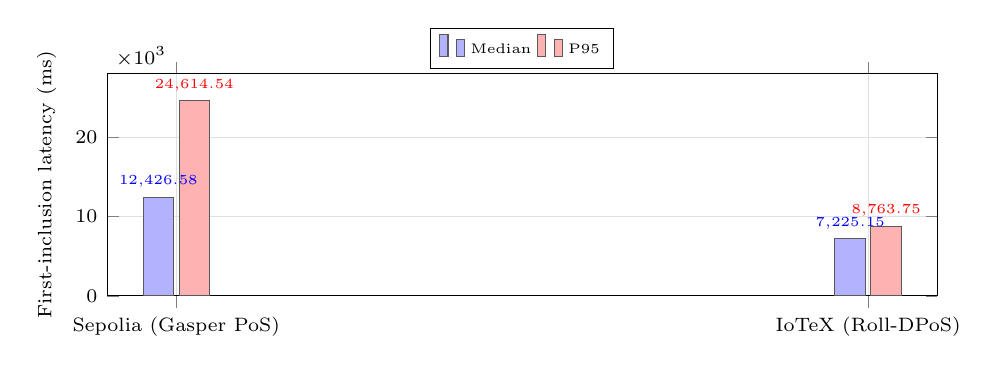
\begin{tikzpicture}
\begin{axis}[width=\columnwidth,height=4.4cm,ybar,bar width=11pt,
ymin=0,ymax=28000,ylabel={First-inclusion latency (ms)},
symbolic x coords={Sepolia (Gasper PoS),IoTeX (Roll-DPoS)},xtick=data,
scaled y ticks=base 10:-3,ytick scale label code/.code={$\times 10^{3}$},
tick label style={font=\scriptsize},label style={font=\scriptsize},
legend style={font=\tiny,at={(0.5,1.02)},anchor=south,legend columns=-1},
nodes near coords,every node near coord/.append style={font=\tiny,rotate=0},
grid=major,major grid style={black!12}]
\addplot+[draw=black!65] coordinates
{({Sepolia (Gasper PoS)},12426.58) ({IoTeX (Roll-DPoS)},7225.15)};
\addplot+[draw=black!65] coordinates
{({Sepolia (Gasper PoS)},24614.54) ({IoTeX (Roll-DPoS)},8763.75)};
\legend{Median,P95}
\end{axis}
\end{tikzpicture}
\caption{Measured first-inclusion latency for matched, concurrently submitted
audit-anchor transactions on the two networks with deployment evidence.
RPC/client overhead and prevailing public-testnet load are included; economic
finality is not measured. The separate Raft/QBFT experiment in
Fig.~\ref{fig:consensus-protocols} uses local permissioned clusters and
different within-family workloads; its absolute latency is not compared with
these public-testnet values.}
\label{fig:paired-latency}
\end{figure}
\subsection{Consensus-Family and SHA-2 Evidence-Anchor Extension}
\label{sec:consensus-extension}
The requested comparison separates two independent design layers: the
consensus protocol that orders an EVM transaction and the cryptographic hash
function that binds the evidence. SHA-256 and SHA-512 are one-way hashes, not
encryption; frozen validation vectors are retained in the
artifact~\cite{artifactRepo}. The Sepolia lane is classified as Gasper PoS
from the network and deployment
evidence~\cite{ethereumNetworks,artifactRepo}. IoTeX uses Roll-DPoS, including
elected delegates, randomised committee formation, and PBFT-style
finalisation~\cite{iotexRollDpos}. The existing public-testnet measurements
therefore remain correctly labelled as a Sepolia--IoTeX
consensus-sensitivity study rather than a controlled causal benchmark of
consensus alone.
Fig.~\ref{fig:consensus-protocols} separates four \emph{measured} lanes
without conflating their estimands. Gasper PoS and Roll-DPoS carry 90 matched
public-testnet first-inclusion pairs. Raft carries local etcd replicated-write
and leader/majority-loss observations, while Besu QBFT carries local EVM
audit-anchor and validator-quorum observations. Raft commits through a
majority quorum and addresses crash faults~\cite{ongaro2014raft}; QBFT requires
a supermajority of approved validators and has a Byzantine protocol fault
model~\cite{besuQbft}. Our interventions, however, stop processes and remove
participation only. Accordingly, the measured QBFT evidence establishes
progress at 3/4, no progress at 2/4, and bounded operator-assisted recovery;
it does not experimentally establish resistance to equivocation or forged
votes.
\begin{figure*}[!t]
\centering
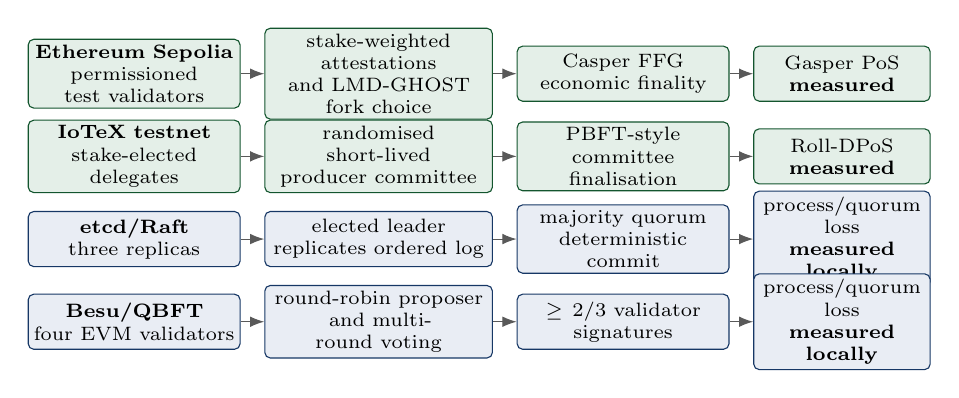
\begin{tikzpicture}[
  lane/.style={draw,rounded corners=2pt,minimum height=7mm,align=center,
               font=\scriptsize,inner sep=2pt},
  measured/.style={lane,fill=trustgreen!12,draw=trustgreen!70!black},
  permissioned/.style={lane,fill=trustblue!10,draw=trustblue!70!black},
  arrow/.style={-{Latex[length=1.8mm]},thin,draw=black!65}
]
\node[measured,text width=2.55cm] (s1) at (0,0)
  {\textbf{Ethereum Sepolia}\\permissioned test validators};
\node[measured,text width=2.75cm,right=3mm of s1] (s2)
  {stake-weighted attestations\\and LMD-GHOST fork choice};
\node[measured,text width=2.55cm,right=3mm of s2] (s3)
  {Casper FFG\\economic finality};
\node[measured,text width=2.1cm,right=3mm of s3] (s4)
  {Gasper PoS\\\textbf{measured}};
\node[measured,text width=2.55cm] (i1) at (0,-1.05)
  {\textbf{IoTeX testnet}\\stake-elected delegates};
\node[measured,text width=2.75cm,right=3mm of i1] (i2)
  {randomised short-lived\\producer committee};
\node[measured,text width=2.55cm,right=3mm of i2] (i3)
  {PBFT-style committee\\finalisation};
\node[measured,text width=2.1cm,right=3mm of i3] (i4)
  {Roll-DPoS\\\textbf{measured}};
\node[permissioned,text width=2.55cm] (r1) at (0,-2.10)
  {\textbf{etcd/Raft}\\three replicas};
\node[permissioned,text width=2.75cm,right=3mm of r1] (r2)
  {elected leader\\replicates ordered log};
\node[permissioned,text width=2.55cm,right=3mm of r2] (r3)
  {majority quorum\\deterministic commit};
\node[permissioned,text width=2.1cm,right=3mm of r3] (r4)
  {process/quorum loss\\\textbf{measured locally}};
\node[permissioned,text width=2.55cm] (q1) at (0,-3.15)
  {\textbf{Besu/QBFT}\\four EVM validators};
\node[permissioned,text width=2.75cm,right=3mm of q1] (q2)
  {round-robin proposer\\and multi-round voting};
\node[permissioned,text width=2.55cm,right=3mm of q2] (q3)
  {$\geq 2/3$ validator\\signatures};
\node[permissioned,text width=2.1cm,right=3mm of q3] (q4)
  {process/quorum loss\\\textbf{measured locally}};
\foreach \a/\b in {s1/s2,s2/s3,s3/s4,i1/i2,i2/i3,i3/i4,
                    r1/r2,r2/r3,r3/r4,q1/q2,q2/q3,q3/q4}
  \draw[arrow] (\a) -- (\b);
\end{tikzpicture}
\caption{Consensus-protocol evidence map extending
Fig.~\ref{fig:paired-latency}. Green lanes are measured public-testnet
first-inclusion configurations; blue lanes are measured local permissioned
clusters. The Raft and QBFT interventions cover process
crash/non-participation, quorum loss, and recovery. They do not inject
equivocation, forged votes, state corruption, or arbitrary Byzantine
messages, and absolute latency is not ranked across unlike workloads.}
\label{fig:consensus-protocols}
\end{figure*}
\begin{table}[!t]
\centering
\caption{Measured permissioned process-loss experiment; latency comparisons
are within implementation because the workloads differ.}
\label{tab:permissioned-fault-results}
\footnotesize
\setlength{\tabcolsep}{3.5pt}
\begin{adjustbox}{width=\columnwidth}
\begin{tabular}{lrrrl}
\toprule
Condition & $n$ & Median (ms) & P95 (ms) & Outcome \\
\midrule
\multicolumn{5}{l}{\emph{etcd/Raft (key/value replicated writes)}} \\
\quad Healthy baseline & 90 & 12.02 & 16.22 & writes committed \\
\quad One follower offline & 90 & 10.25 & 12.68 & writes committed \\
\quad After leader failover & 90 & 10.43 & 14.46 & writes committed \\
\quad Majority unavailable & 90 & -- & -- & 90/90 rejected \\
\midrule
\multicolumn{5}{l}{\emph{Besu/QBFT (EVM audit anchors)}} \\
\quad Healthy baseline & 90 & 4{,}101.1 & 4{,}116.6 & anchors included \\
\quad One validator offline (3/4) & 90 & 4{,}100.1 & 8{,}117.0 & anchors included \\
\quad Two validators offline (2/4) & 90 & -- & -- & 90/90 no progress \\
\quad Recovered cluster (4/4) & 90 & 4{,}105.2 & 8{,}126.7 & anchors included \\
\bottomrule
\end{tabular}
\end{adjustbox}
\end{table}
Across the three sessions, median observed Raft leader-failover recovery was
1{,}125.9\,ms; operator-assisted QBFT restoration resumed production after
14{,}649.7\,ms. All sessions passed their SHA-256 manifests and derivation
gate and are retained in the artifact~\cite{artifactRepo}. Absolute Raft and
QBFT latencies are not ranked because their operations differ.
The SHA-2 comparison is bounded by a fairness rule: both algorithms hash
identical retained payload bytes and anchor their complete digest through
identical \texttt{HashCommitmentLedger} runtime bytecode. SHA-256 (256-bit
digest, 512-bit message block, 32-bit words, $\approx$128-bit generic
collision work) anchors one 32-byte full digest and also has a standard EVM
precompile; SHA-512 (512-bit digest, 1024-bit message block, 64-bit words,
$\approx$256-bit generic collision work) has no standard EVM precompile, so it
is computed off chain and anchors one 64-byte full
digest~\cite{artifactRepo}. Both digests are computed off chain in the
primary comparison, which isolates digest-width, calldata, event, and storage
effects from CPU hash throughput. Solidity provides a SHA-256
precompile-backed built-in, whereas the standard EVM does not provide an
equivalent SHA-512 precompile in the evaluated path~\cite{artifactRepo}. A
separate \texttt{computeSha256AndAnchor} entry point can measure the SHA-256
precompile path, but that result is not presented as a symmetric SHA-256
versus SHA-512 computation benchmark.
\paragraph{Validated local hash-primitive reference}
An isolated Hardhat contract separately compares the Keccak-256 opcode path,
the SHA-256 precompile path, and a FIPS-vector-gated pure-Solidity SHA-512
implementation for deterministic 32-byte and 1{,}024-byte inputs. After three
excluded warm-ups, 30 \texttt{eth\_call} observations are retained per
algorithm/input cell with cyclically balanced order. The local hash
publication gate passed all retained-payload digest checks and the
SHA-256/SHA-512 validation vectors. For the 32-byte input, the median
primitive-path deltas were 59 gas for Keccak-256, 392 gas for the SHA-256
precompile path, and 162{,}174 gas for the pure-Solidity SHA-512 reference.
For the 1{,}024-byte input, the median primitive-path deltas were 245 gas for
Keccak-256, 2{,}879 gas for the SHA-256 precompile path, and 1{,}614{,}065 gas
for the pure-Solidity SHA-512 reference
(Table~\ref{tab:hash-primitive-microbenchmark},
Fig.~\ref{fig:composite-cost-stress}(a)). All 30 calls per
algorithm/input cell returned the same delta because the bytecode, input, and
local EVM state were fixed. The reported \texttt{gasleft()} deltas are
specific to Solidity 0.8.20, optimizer 200, \texttt{viaIR=true}, and the Paris
EVM target. The pure-Solidity SHA-512 implementation is an experimental
instrument only; the deployable workflow computes SHA-512 off chain and
anchors its complete 64-byte digest.
\begin{table}[!t]
\centering
\caption{Validated local hash-primitive measurements.}
\label{tab:hash-primitive-microbenchmark}
\small
\begin{tabular}{lrrrr}
\toprule
Primitive & Bytes & Median gas & $n$ & Fixed \\
\midrule
Keccak-256 & 32 & 59 & 30 & yes \\
SHA-256 & 32 & 392 & 30 & yes \\
SHA-512 (Solidity) & 32 & 162{,}174 & 30 & yes \\
Keccak-256 & 1{,}024 & 245 & 30 & yes \\
SHA-256 & 1{,}024 & 2{,}879 & 30 & yes \\
SHA-512 (Solidity) & 1{,}024 & 1{,}614{,}065 & 30 & yes \\
\bottomrule
\end{tabular}
\end{table}
Interpretation of the public-testnet, permissioned-fault, and hash results
follows the single Claim Boundary in Section~\ref{sec:claim-boundary}.
\subsection{Stage 3 KPI Evidence-Field Coverage}
Anchor gas, policy-reasoning latency, replay rejection, zero-anchor rejection,
unauthorised-submitter rejection, and gas logs are present in all 240 rows.
Coverage denotes field capture, not security effectiveness. The later ZK
audit supersedes the earlier interpretation of a prover-time field: the matrix
contains no row-bound proof outcome or proof/public-input binding, so no
successful per-row verification is inferred.
Stage~3 uses the isolated \texttt{Stage3AnomalyLedger} micro-benchmark to
emit direct evidence for anchor gas and negative-security behaviour (duplicate,
zero, and unauthorised-submitter rejection) plus a deterministic per-run
policy-reasoning latency probe; Stages~4--5 strengthen this externally through
the Sepolia deployment and the paired Sepolia--IoTeX design with its strict
publication gate, without turning the micro-benchmark into a production trust
ledger.
\subsection{AUTH\_V2.2 Timing and Proof Boundary}
\label{sec:auth-boundary}
The paper-specific hardening workflow adds a self-healing local AUTH\_V2.2
timing path: it checks dependencies, starts Hardhat when required, compiles
artifacts, redeploys when the stored address has no bytecode, and then measures
the verifier-call runner. Because the hardened run returned
\texttt{verifyTx=false}, the observation is only verifier-call timing smoke
evidence on an ephemeral chain. A read-only audit found no per-row proof
outcome or proof/public-input binding in the frozen matrix: the full-system
and no-IPFS variants each have 40/40 missing prover-time records, while the
other four variants record that the prover was not invoked. Constant verifier
gas is not validity evidence. The matrix therefore supports 0/240 row-bound
successful verifications; AUTH\_V2.2 is only a component experiment.
\subsection{Configured Profile Stress}
Fig.~\ref{fig:composite-cost-stress}(b) summarises the full-system profile
trend. The
configured clean-to-delay+jitter+loss profiles increase end-to-end duration,
whereas the reasoning probe stays within a narrow millisecond-scale
range. Thus audit micro-benchmark gas logic is independent of media-profile
configuration, while workflow duration reflects the configured impairment.
\begin{figure*}[t]
\centering
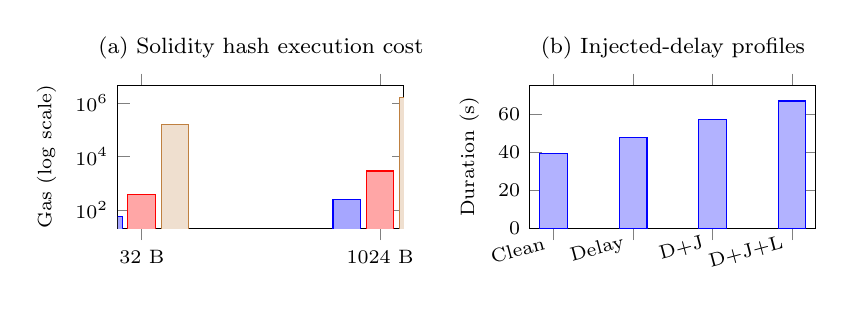
\begin{tikzpicture}
\begin{groupplot}[
  group style={group size=2 by 1,horizontal sep=1.6cm},
  width=.43\textwidth,height=.28\textwidth,ybar,
  tick label style={font=\scriptsize},label style={font=\scriptsize},
  title style={font=\footnotesize},legend style={font=\scriptsize,draw=none}
]
\nextgroupplot[title={(a) Solidity hash execution cost},
  symbolic x coords={32 B,1024 B},xtick=data,ylabel={Gas (log scale)},
  ymode=log,log basis y=10]
  \addplot[fill=blue!35,draw=blue] coordinates {(32 B,59) (1024 B,245)};
  \addplot[fill=red!35,draw=red] coordinates {(32 B,392) (1024 B,2879)};
  \addplot[fill=brown!25,draw=brown] coordinates {(32 B,162174) (1024 B,1614065)};
\nextgroupplot[title={(b) Injected-delay profiles},
  symbolic x coords={Clean,Delay,D+J,D+J+L},xtick=data,
  x tick label style={rotate=15,anchor=east},ylabel={Duration (s)},ymin=0,ymax=75]
  \addplot coordinates {(Clean,39.06) (Delay,47.44) (D+J,56.88) (D+J+L,66.82)};
\end{groupplot}
\end{tikzpicture}
\par\smallskip
{\scriptsize (a) \textcolor{blue}{Keccak-256}; \textcolor{red}{SHA-256};
\textcolor{brown}{SHA-512}. \quad (b) Configured end-to-end duration.}
\caption{\rev{Hash cost and configured stress results. The panels have distinct
workloads and are not an end-to-end deployment comparison.}}
\label{fig:composite-cost-stress}
\end{figure*}


\begin{revision}
\subsection{Retained Output Ablation and Timing Attribution}
\label{sec:retained-ablation}
We replayed the unchanged 180 LangGraph and 60 Qwen records through
(i) their raw candidate output, (ii) the recorded class-consistency guard
and (iii) that guard with automatic execution administratively disabled.
The last intervention changes only \texttt{execute}, never the decision,
action class or oracle labels. Table~\ref{tab:output-ablation} therefore tests
the distinction between semantic agreement and execution declarations.
\begin{table}[!t]
\centering\ifshowrevisions\color{blue}\else\color{black}\fi\footnotesize
\caption{\rev{Paired output replay. D/A are decision/action agreement counts;
E is execute-true declarations; N is the subset on oracle-NEVER cells.
No network action or new model call is measured.}}
\label{tab:output-ablation}
\begin{tabular}{llrrrr}
\toprule Records & Processing & D & A & E & N \\
\midrule
LangGraph (180) & Raw & 150 & 120 & 0 & 0 \\
 & Class guard & 150 & 120 & 0 & 0 \\
 & Execution disabled & 150 & 120 & 0 & 0 \\
Qwen (60) & Raw & 38 & 11 & 38 & 9 \\
 & Class guard & 38 & 11 & 38 & 9 \\
 & Execution disabled & 38 & 11 & 0 & 0 \\
\bottomrule
\end{tabular}
\end{table}
All six reference scenarios require HUMAN or NEVER handling. Thus disabling
execution makes this declaration metric zero without improving any semantic
label or demonstrating useful automatic service. The benchmark cannot by
itself establish correctness, actuation safety or the value of an always-block
policy. The proposed workflow's original zero unsafe-automatic count is a
reported gate outcome under its synthetic configuration, distinct from the
baseline prediction flags and the single approved simulated write.

One retained S2 trace permits a limited timing explanation. Its internal
timestamps span 108.939~s: input to frozen retrieval, 4.380~s; retrieval to
provider aggregate, 26.876~s; aggregate through the four-role chain,
77.573~s; final reflection to report, 0.109~s. Parallel provider wall time is
25.421~s, while summed provider calls are 42.896~s; these overlap and must not
be added to the wall intervals. Summed role calls are 77.397~s. These values
identify the expensive stages in that one trace, excluding subsequent human
waiting; they do not decompose the 180-cell median or isolate a causal
LangGraph/n8n difference. The 109.436~s n8n envelope includes additional
orchestration outside the internal report timestamps.
\end{revision}

\begin{revision}
\subsection{Scientific Interpretation and Limitations}
The evidence classes have different estimands and denominators. Runtime hooks,
finite-state counts, frozen oracle cells, matched testnet transactions, and
configured impairment profiles must not be combined into one system score.
The configured LangGraph comparison does not isolate the latency cost of
provider diversity, agent roles or governance; the Qwen3-4B result
shows that local reproducibility alone does not guarantee oracle-conformant classification.
The prompt-injection suite tests only 30 synthetic variants.
The R10 endpoints used the recorded aliases \texttt{gpt-5.6-terra},
\texttt{claude-fable-5}, \texttt{deepseek-v4-pro}, and
\texttt{mistral-medium-3-5} on 16 July 2026; immutable provider snapshots were
not exposed. Temperature, top-$p$, and top-$k$ were unsent, so no defaults are
inferred. The maximum-output field was 5{,}000 tokens for OpenAI, Anthropic,
and Mistral and was omitted for DeepSeek. Prompt hashes match all 180 cells;
full prompts and the sent-field inventory are in the supplement.
\paragraph{Future independent human validation}
Independent expert validation was not completed. A future study requires eligible independent O-RAN-literate annotators and
any applicable institutional review. The frozen oracle will remain unchanged.
Decision and action categories should be treated as nominal, with unweighted
agreement statistics and whole-scenario resampling. The archived protocol's
weighted action statistic assumes an ordering that the four authority classes
do not establish; it must be amended and frozen before collecting new labels.
No amended study or human agreement statistic is reported here.
\end{revision}

\begin{revision}
\section{Conclusion and Future Directions}
\label{sec:conclusion}
This paper addressed a practical governance question: how can large-language-
model assistance be introduced into O-RAN security operations without allowing
the model to become the enforcement authority? The proposed two-plane
architecture separates observation and reasoning from deterministic policy,
operator approval, and evidence services. A recommendation therefore remains a
proposal until the four-class action ladder accepts, escalates, or rejects it.
Hash-bound lineage connects the input, retrieved evidence, model proposals,
final decision, approval record, and audit receipt, while the architecture
contains no direct model-to-E2 actuation path. This makes the intended role
explicit: decision support for non-real-time policy loops, not autonomous
near-real-time radio control.

The evaluation provides complementary evidence rather than a single aggregate
score. Formal model checking covered all 320 states of the configured
policy-gate abstraction and found no violation of six safety rules. On the
frozen 180-case benchmark, the proposed workflow achieved 100.0\% decision
agreement and 96.7\% action agreement, compared with 83.3\% and 66.7\% for the
external LangGraph baseline; both reported zero unsafe automatic flags under their respective benchmark definitions. The local
Qwen3-4B run shows that reproducible deployment alone does not guarantee safe
classification, and the 30-case injection suite supports only bounded
containment claims. Across 90 matched transaction pairs, median inclusion time
was 12.427~s on Sepolia and 7.225~s on IoTeX, while the live n8n workflow wrote
only to a simulated ledger after explicit human approval. These configured workflows differ simultaneously in reasoning, request budgets
and governance. The replay ablation separates execution declarations from
semantic agreement; the 80.5--109.8~s median durations do not isolate a
framework or component cost.

The claims remain limited to the released artifacts, a synthetic frozen
oracle, public testnets, local permissioned clusters, and simulated actuation.
The study does not establish production O-RAN safety, semantic correctness of
model output, or system-level zero-knowledge verification; the retained matrix
supports no row-bound successful proof verification. Future work will validate
the oracle with the preregistered independent-annotator protocol, add
production-derived scenarios and multiple client/RPC vantage points, exercise
arbitrary-Byzantine and adaptive multi-turn attacks, and implement row-bound
proof/public-input binding. Standard A1 payloads, tighter SMO/Non-RT RIC
integration, and lower latency can then support fail-closed operator pilots.
\end{revision}
% \section*{Data and Artifact Availability}
% Source code, workflows, machine-readable measurements, prompts, validation
% scripts, and SHA-256 manifests are available at
% \url{https://github.com/Sudarson2021/zktrustllm-agents-l4}. The frozen
% version~1.0.0 release is archived on Zenodo under DOI
% 10.5281/zenodo.21939774~\cite{artifactRepo}. Public testnet transaction
% identifiers permit independent receipt checks. API credentials, provider-side
% logs, and personal data are not distributed.
\section*{Acknowledgment}
This work is supported by the CHEDDAR (Communications Hub for Empowering
Distributed Cloud Computing Applications and Research) programme under UK
EPSRC grants EP/Y037421/1 and EP/X040518/1, and by the Open Challenge Fund
call organised by the Datacom Industry Association AISBL. Also, the ADU author
acknowledges support from Abu Dhabi University's Office of Research and Grant Programs.
\rev{OpenAI Codex assisted with drafting revision additions to Sections~II,
IV--VIII and the supplement, preparing deterministic reanalysis and formal-check
scripts, and reconstructing editable workflow figures from archived exports.
This assistance generated no new experimental model responses or human labels.
Responsibility for the final content and validation rests with the authors.}

% Keep the IEEE 8-pt reference font but use an 8.8-pt baseline and a small,
% uniform inter-entry reduction while preserving a readable bibliography in the revised layout.
% IEEEtran calls \footnotesize inside thebibliography, so redefine only this
% end-of-document instance rather than changing the manuscript body.
\renewcommand{\footnotesize}{\fontsize{8}{8.8}\selectfont}
\def\IEEEbibitemsep{-0.25pt plus .1pt}
\begin{thebibliography}{40}
\bibitem{nistZeroTrust}
S. Rose, O. Borchert, S. Mitchell, and S. Connelly, ``Zero Trust
Architecture,'' NIST Special Publication 800-207, 2020.
\bibitem{oranA1}
O-RAN Software Community, ``A1 mediator documentation,'' 2023. [Online].
Available: \url{https://docs.o-ran-sc.org/}
\bibitem{oranSecReq}
ETSI, ``O-RAN security requirements and controls specifications,'' ETSI
TS~104~104 V9.1.0 (O-RAN.WG11.SecReqSpecs-R003-v09.01), Jun. 2025.
\bibitem{oranSecProtocols}
ETSI, ``O-RAN security protocols specifications,'' ETSI TS~104~107 V9.0.0
(O-RAN.WG11.Security-Protocols-Specification.O-R003-v09.00), May 2025.
\bibitem{oranThreatModel}
ETSI, ``O-RAN security threat modeling and risk assessment,'' ETSI
TR~104~106 V3.0.0 (O-RAN.WG11.Threat-Modeling.O-R003-v03.00), Jun. 2025.
\bibitem{threegpp33501}
3GPP, ``Security architecture and procedures for 5G system,'' 3GPP
TS~33.501 V18.12.0, Release~18, Jul. 2026.
\bibitem{groth16}
J. Groth, ``On the size of pairing-based non-interactive arguments,'' in
\emph{Proc. EUROCRYPT}, 2016, pp. 305--326.
\bibitem{lamportTla}
L. Lamport, \emph{Specifying Systems: The TLA\textsuperscript{+} Language and
Tools for Hardware and Software Engineers}. Boston, MA, USA: Addison-Wesley,
2002.
\bibitem{chatzimiltis2026}
S. Chatzimiltis, M. Boloursaz Mashhadi, M. Shojafar, M. Debbah, and
R. Tafazolli, ``Agentic AI for 6G: A new paradigm for autonomous RAN security
compliance,'' \emph{IEEE Commun. Standards Mag.}, early access, Apr. 2026,
doi: 10.1109/MCOMSTD.2026.3681685.
\bibitem{he2026agentic}
Z. He \emph{et al.}, ``Agentic AI-RAN: Enabling intent-driven, explainable and
self-evolving Open RAN intelligence,'' arXiv:2602.24115v2, 2026. [Online].
Available: \url{https://arxiv.org/abs/2602.24115}
\bibitem{elkael2025agentran}
M. Elkael \emph{et al.}, ``AgentRAN: An agentic AI architecture for autonomous
control of open 6G networks,'' \emph{IEEE Commun. Mag.}, early access, 2026,
doi: 10.1109/MCOM.001.2500563.
\bibitem{navidan2026}
H. Navidan \emph{et al.}, ``Toward autonomous O-RAN: A multi-scale agentic AI
framework for real-time network control and management,'' \emph{IEEE
Network}, early access, 2026, doi: 10.1109/MNET.2026.3701847.
\bibitem{santos2024xapp}
J. F. Santos \emph{et al.}, ``Managing O-RAN networks: xApp development from
zero to hero,'' arXiv:2407.09619, 2024.
\bibitem{n8nDocs}
n8n, ``Workflows, nodes, and integrations documentation,'' 2026. [Online].
Available: \url{https://docs.n8n.io/}
\bibitem{langchainDocs}
LangChain, ``LangChain and LangGraph documentation,'' 2026. [Online].
Available: \url{https://docs.langchain.com/}
\bibitem{qwen3}
Qwen Team, ``Qwen3: Open-weight large language model family,'' 2025.
[Online]. Available: \url{https://github.com/QwenLM/Qwen3}
\bibitem{crewaiDocs}
CrewAI, ``CrewAI documentation,'' 2026. [Online]. Available:
\url{https://docs.crewai.com/}
\bibitem{wu2023autogen}
Q. Wu \emph{et al.}, ``AutoGen: Enabling next-gen LLM applications via
multi-agent conversation,'' arXiv:2308.08155, 2023.
\bibitem{li2023camel}
G. Li, H. A. K. Hammoud, H. Itani, D. Khizbullin, and B. Ghanem, ``CAMEL:
Communicative agents for `mind' exploration of large language model society,''
arXiv:2303.17760, 2023.
\bibitem{ethereumNetworks}
Ethereum Foundation, ``Networks: Ethereum testnets and Sepolia,'' 2026.
[Online]. Available: \url{https://ethereum.org/developers/docs/networks/}
\bibitem{iotexRollDpos}
IoTeX Foundation, ``Roll-DPoS consensus,'' 2025. [Online]. Available:
\url{https://docs.iotex.io/blockchain/learn-iotex/core-concepts/}
\bibitem{iotexRpc}
IoTeX Foundation, ``RPC endpoints: IoTeX mainnet and testnet,'' 2026.
[Online]. Available: \url{https://docs.iotex.io/}
\bibitem{artifactRepo}
S. Karmaker, M. Shojafar, and H. S. Cruickshank, ``Reproducibility artifact
for auditable policy-governed LLM-agent control for O-RAN edge security,''
Zenodo, version 1.0.0, Aug. 14, 2026, doi: 10.5281/zenodo.21939774.
\bibitem{ongaro2014raft}
D. Ongaro and J. Ousterhout, ``In search of an understandable consensus
algorithm,'' in \emph{Proc. USENIX Annu. Tech. Conf. (ATC)}, 2014,
pp. 305--319.
\bibitem{besuQbft}
Hyperledger Besu, ``QBFT consensus protocol documentation,'' 2026. [Online].
Available: \url{https://besu.hyperledger.org/}
\bibitem{karmakerZktrustllmIccw26}
S. Karmaker, H. Cruickshank, and M. Shojafar, ``ZKTrustLLM: IPFS-anchored
zero-knowledge accountability for secure 5G/O-RAN edge multicast,'' in
\emph{Proc. IEEE Int. Conf. Commun. Workshops (ICC Workshops)}, 2026, doi:
10.1109/ICCWorkshops63917.2026.11586313.
\bibitem{lin2025ztric}
D. Lin, T. Do, A. Herath, M. Shirazipour, and V. K. Shah, ``ZT-RIC: A zero
trust RIC framework for ensuring data privacy and confidentiality in Open
RAN,'' in \emph{Proc. IEEE Consum. Commun. Netw. Conf. (CCNC)}, 2025.
\bibitem{abdalla2024ztran}
A. S. Abdalla, J. Moore, N. Adhikari, and V. Marojevic, ``ZTRAN: Prototyping
zero trust security xApps for Open Radio Access Network deployments,''
arXiv:2403.04113, 2024.
\bibitem{nahar2024zta}
N. Nahar, K. Andersson, O. Schel{\'e}n, and S. Saguna, ``A survey on zero
trust architecture: Applications and challenges of 6G networks,'' \emph{IEEE
Access}, vol. 12, pp. 94753--94764, 2024.
\bibitem{aleisa2025blockchain}
M. A. Aleisa, ``Blockchain-enabled zero trust architecture for
privacy-preserving cybersecurity in IoT environments,'' \emph{IEEE Access},
vol. 13, pp. 18660--18676, 2025.
\bibitem{zhou2025llmtelecom}
H. Zhou, C. Hu, Y. Yuan \emph{et al.}, ``Large language model (LLM) for
telecommunications: A comprehensive survey on principles, key techniques, and
opportunities,'' \emph{IEEE Commun. Surveys Tuts.}, vol. 27, no. 3,
pp. 1955--2005, 2025.
\bibitem{boateng2025llm}
G. O. Boateng \emph{et al.}, ``A survey on large
language models for communication, network, and service management:
Application insights, challenges, and future directions,'' \emph{IEEE Commun.
Surveys Tuts.}, \rev{vol. 28, pp. 527--566, 2026, doi: 10.1109/COMST.2025.3564333.}
\bibitem{long2025llmops}
S. Long, J. Tan, B. Mao \emph{et al.}, ``A survey on intelligent network
operations and performance optimization based on large language models,''
\emph{IEEE Commun. Surveys Tuts.}, \rev{vol. 27, no. 6,
pp. 3915--3949, Dec. 2025}, doi: 10.1109/COMST.2025.3526606.
\bibitem{ramezanpour2022izta}
K. Ramezanpour and J. Jagannath, ``Intelligent zero trust architecture for
5G/6G networks: Principles, challenges, and the role of machine learning in
the context of O-RAN,'' \emph{Comput. Netw.}, vol. 217, p. 109358, 2022.

\begin{revision}
\bibitem{oranalyst2024} T. Yang, S. M. M. Rashid, A. Ranjbar, G. Tan, and
S. R. Hussain, ``ORANalyst: Systematic testing framework for Open RAN
implementations,'' in \emph{Proc. USENIX Security}, 2024, pp. 1921--1938.
\bibitem{invaran2026} T. Yang, A. Ranjbar, G. Tan, and S. R. Hussain,
``Invariant-guided logical testing of Open RAN controllers,'' in
\emph{Proc. USENIX Security}, 2026, pp. 711--730.
\bibitem{veraran2026} Y. Hou and Z. Yang, ``VeraRAN: Pre-actuation certification
and event-causal synchronization repair for asynchronous multi-interface RAN
plans,'' arXiv:2608.01047v3, Aug. 2026.
\bibitem{safetycopilot2026} M. A. Jawad, M. M. H. Munna, A. H. Kabir,
N. H. Antu, and R. F. Tulona, ``A runtime safety copilot for AI-native O-RAN:
Predictive verification and fail-safe enforcement in near-RT RIC control
loops,'' \emph{IEEE Access}, vol. 14, pp. 63106--63120, 2026,
doi: 10.1109/ACCESS.2026.3686132.
\bibitem{multilayer2026} H. Alimohammadi, S. Mayhoub, S. Chatzimiltis,
M. Shojafar, and M. N. M. Bhutta, ``Toward a multi-layer defence framework
for securing near-real-time operations in Open RAN,'' \emph{IEEE Open J.
Commun. Soc.}, vol. 7, pp. 480--497, 2026,
doi: 10.1109/OJCOMS.2025.3650736. Accepted-version text:
arXiv:2512.01596v2.
\bibitem{salmi2026tnsm} S. Salmi \emph{et al.}, ``AI-native O-RAN
architectures for 6G: Toward real-time adaptation, conflict resolution,
and efficient resource management,'' \emph{IEEE Trans. Netw. Service Manag.},
vol. 23, pp. 4110--4121, 2026, doi: 10.1109/TNSM.2026.3684880.
\end{revision}
\end{thebibliography}
% \begin{IEEEbiography}[{\includegraphics[width=1in,height=1.25in,clip,
% keepaspectratio]{figures/author_sudarson_karmaker.jpg}}]{Sudarson Karmaker}
% is a researcher at the Institute for Communication Systems, University of
% Surrey, Guildford, U.K. His research interests include O-RAN security,
% zero-trust networking, distributed ledgers, and auditable agentic AI for
% communication networks.
% \end{IEEEbiography}
% \begin{IEEEbiography}[{\includegraphics[width=1in,height=1.25in,clip,
% keepaspectratio]{figures/author_mohammad_shojafar.png}}]{Mohammad Shojafar}
% is an Associate Professor in network security at the Institute for
% Communication Systems, University of Surrey, Guildford, U.K. He received the
% Ph.D. degree from Sapienza University of Rome, Italy, in 2016. His research
% interests include network security, distributed systems, edge computing, and
% resource management. He is a Senior Member of the IEEE and a Fellow of the
% Higher Education Academy.
% \end{IEEEbiography}
% \begin{IEEEbiography}[{\includegraphics[width=1in,height=1.25in,clip,
% keepaspectratio]{figures/author_haitham_cruickshank.png}}]{Haitham S. Cruickshank}
% is a Reader at the Institute for Communication Systems, University of Surrey,
% Guildford, U.K. His research interests include network, user, and Internet of
% Things security and privacy, with applications to mobile, satellite, and
% Internet communications.
% \end{IEEEbiography}
\end{document}
